% !TeX root = ../sustechthesis-example.tex

\chapter[基于FPGA的RTMQ测控系统]{基于FPGA的RTMQ测控系统\label{section:fpga_rtmq}}

% \textcolor{red}{
% 这部分参考RTMQ的相关专利和文档介绍整个测控系统的情况... 
% }
\section[实时系统]{实时系统}

量子物理实验系统常常涉及到一些物理量的精确调控和测量,这既包括量上的精确性,也包括时间上的精确性。因此量子物理实验系统对测量和控制性能提出了很多新的要求,其中十分关键的一点就是对测控系统实时性的要求。

现有的实时系统一般使用主频在数百MHz至GHz量级的通用微处理器或微控制器作为控制的主体,以计时器中断和时间片分配等方式实现实时控制。这一方案成立的前提在于,所需的时间控制精度与指令执行频率之间有3-6个数量级的差异,因而通用处理器架构中存在的一些诸如分支预判、乱序执行等导致指令执行顺序不确定的因素以及中断系统中存在的现场保护、控制权交接等额外开销导致的时间控制不确定性可以忽略不计。

然而近来随着量子技术的发展,量子物理实验系统也开始产生对数据处理、复杂流程控制和实时控制的需求。不同于传统行业,量子物理实验系统对时间控制的精度和分辨率的要求在纳秒量级、延迟要求在百纳秒至数十微秒量级,与当前微处理器的主频相当,从而前述的现有的实时控制方案难以满足需求。

因此早年在量子物理实验领域内,通常用FPGA(现场可编程门阵列)设计特定的时序脉冲发生器来产生高时间精度的脉冲序列,以此作为其它实验设备的触发信号,进行准确的时序控制。然而,这种方案的灵活性较差,只能产生预定的序列,无法在实验中对实验数据进行即时的处理,或根据实验的中间结果对后续的流程进行及时的调整。近年来随着量子算法的发展,实验方案越来越复杂,实验流程中开始包含快速反馈的结构,即在实验过程中对实验目标进行测量,获得一些中间结果,而后对中间结果进行计算和处理,并进而确定后续的实验流程。中间结果的处理和后续流程的确定,一般要求在数十纳秒至数十微秒量级的时间内完成,并且执行时刻必须要严格确定。这要求实验的测控系统具有通用计算的能力,简单的时序脉冲发生器无法满足这一要求。

当前领域内针对此问题的主要解决思路为,另置一与时序脉冲发生器紧密连接的通用微处理器,用来对实验数据进行即时处理和产生时序脉冲发生器的后续输出时序。这一方案能较好的满足系统规模较小且实验时序不太复杂的情形下的实时控制需求。然而,这一方案的问题之一在于,微处理器和时序脉冲发生器依然是相互独立的两个个体,而微处理器的执行时序有其内在不确定性;二者之间要保持同步,或者需要频繁地相互交换触发信号,或者需要在时序设计上预留出充足的余量以覆盖此不确定性的最坏情形,总之都会复杂化时序的设计并产生时间浪费。

这一方案的另一问题在于,当系统规模较大,一个时序脉冲发生器无法控制整个系统时,就需要同时使用多个时序脉冲发生器,而一个微处理器同时处理过多的实验数据、同时控制过多的时序脉冲发生器,将不可避免的产生拥塞,这会进一步加剧前述的同步性问题。而如果同时使用多个微处理器,则不同微处理器之间的同步性又将成为问题;当前主流的微处理器架构和指令集都是针对通用计算而优化的,主流的微处理器使用的通信协议都是针对高吞吐率而优化的,二者都难以实现精确的时序同步。

\section[RTMQ实时系统架构]{RTMQ实时系统架构}

对于离子阱量子计算研究来说,一种实时性更强、拓展性更好、更灵活的测控系统十分重要。我们实验中对系统的控制和测量采用一种叫RTMQ的系统架构来实现。RTMQ系统架构提供了一种新的量子物理实验平台实时测控系统架构,解决了上述的不足。在RTMQ系统架构中,通用计算和时序控制由同一微处理器实现,因此避免了两个独立的模块之间同步性的问题;同时树状结构的系统中每个节点都具有通用计算的能力,因此可以实现计算任务的分布式处理,避免了拥塞的问题。

\begin{figure}
    \centering
    \caption[RTMQ系统架构示意图]{RTMQ系统架构示意图\label{fig:rtmq_nodes_and_leaves_structure}}
    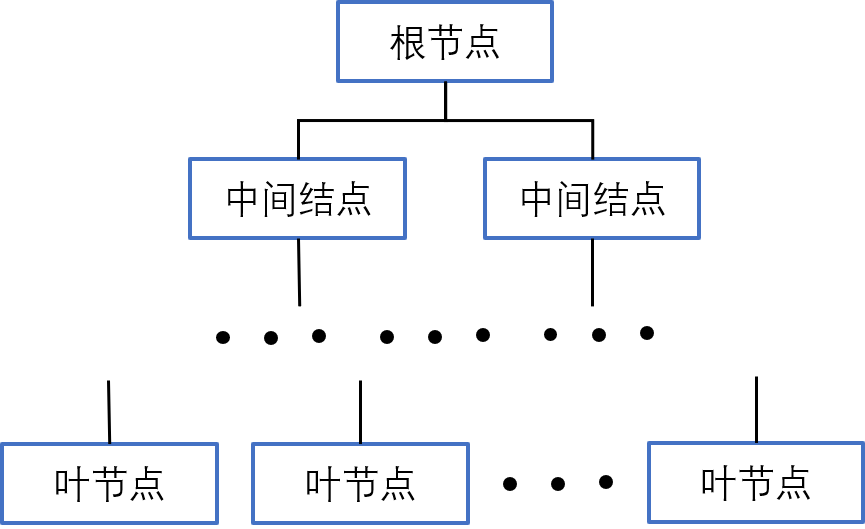
\includegraphics[width=0.6\linewidth]{rtmq/rtmq_nodes_and_leaves_structure}
\end{figure}

RTMQ(用于量子物理实验的实时微系统,RealTime Microsystem for Quantum physics)架构主要用于基于FPGA或ASIC的兼具通用计算和高精度时序控制能力的微系统。系统的整体结构为树状结构,如图\ref{fig:rtmq_nodes_and_leaves_structure}所示,系统包含一个根节点,多个中间结点和多个叶节点;根节点通过网络、USB等方式与控制计算机相连。不同节点可位于同一PCB上,亦可位于不同PCB上。

\begin{figure}
    \centering
    \caption[RTMQ系统架构节点示意图]{RTMQ系统架构节点示意图\label{fig:rtmq_board_overal_structure}}
    
\includegraphics[width=0.4\linewidth]{rtmq/rtmq_board_overal_structure}
\end{figure}

一般而言一个板卡具有如图\ref{fig:rtmq_board_overal_structure}所示的结构,板卡上的FPGA或ASIC包含一个RTMQ节点,RTMQ节点通过控制FPGA或ASIC的输入输出与数模/模数转换等各类功能芯片进行交互以实现所需功能,同时通过实时通信链路与其上级和下级节点连接。

\begin{figure}
    \centering
    \caption[RTMQ系统架构节点内部模块示意图]{RTMQ系统架构节点内部模块示意图\label{fig:rtmq_board_inner_structure}}
    
\includegraphics[width=1.0\linewidth]{rtmq/rtmq_board_inner_structure}
\end{figure}

一个RTMQ节点的内部模块如图\ref{fig:rtmq_board_inner_structure}所示,包含一个32位的微处理器、一个寄存器文件、一系列外设模块和一个链路管理模块。其中微处理器包含流控制器、计时器、异常管理模块、触发管理模块和算术逻辑单元5个子模块;寄存器文件包含多个寄存器;外设可分为系统外设和功能外设,系统外设包括指令缓存、数据缓存、节点信息只读存储器以及地址栈和数据栈,功能外设用于实现具体的逻辑或时序功能,可包含多个。

RTMQ架构中包含的微处理器可受指令控制进入挂起状态,而挂起状态可受计时器或触发管理模块的控制恢复正常运行,如此,微处理器的指令流便可以按一定的时间间隔对齐或与外部信号对齐。同时,节点中的系统外设和功能外设的行为受关联寄存器的读写控制,即微处理器的指令与系统各模块的功能和时序有严格的对应关系。因此,本发明提供的架构可实现实时控制与通用计算在指令流层面的结合。
而配置指令插入中断的机制确保了节点对其下级节点的绝对控制,即使下级节点的微处理器处于挂起状态,依然不受影响。配置指令插入中断配合具有确定通信延迟的实时通信链路系统,即可实现时序确定的跨节点的即时反馈控制。

此外,RTMQ架构中每个节点都具有通用计算和时序控制能力,如此,大多数通用计算和时序生成都可以在叶节点或较近的中间结点完成,对于大规模系统不存在拥塞的问题,具有良好的可扩展性。
% \section[测控硬件组成]{测控硬件组成}
% \textcolor{red}{
% 1. 展示实物板卡照片;}
RTMQ测控板实物图如附录图\ref{fig:rtmq_board_real}所示。
% \begin{figure}
%     \centering
%     \caption[RTMQ测控板实物图]{RTMQ测控板实物图\label{fig:rtmq_board_real}}
%     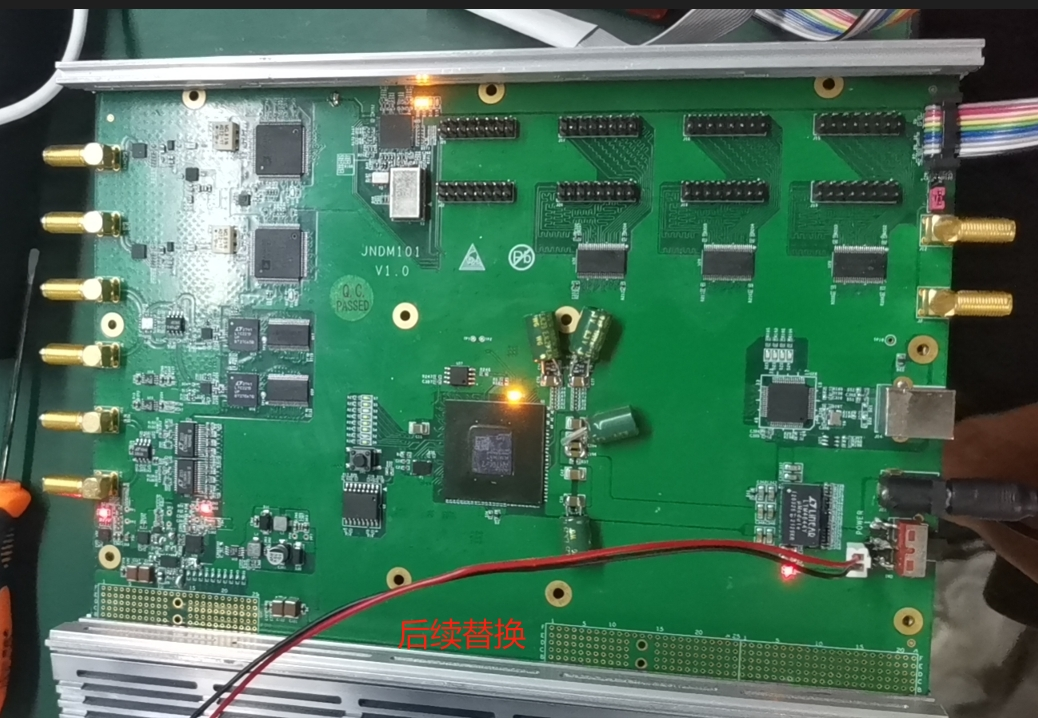
\includegraphics[width=1.0\linewidth]{rtmq/rtmq_board_real}
% \end{figure}

% \textcolor{red}{
% 2. 结合照片给出主要器件清单及其介绍(参考专利:一种量子物理实验平台的实时测控系统架构);}



% \section[软件API]{软件API}
% \textcolor{red}{
% 1. 介绍软件API的功能和使用(可选,根据情况看吧,怎么介绍还没想好);}


\section[基于FPGA的数字超前进位加法器]{基于FPGA的数字超前进位加法器}
% \textcolor{red}{
% 1. 介绍数字加法器功能、逻辑图、Vivado中的实现、局限性;}

\subsection[加法器]{加法器}


加法器是一种用于执行加法运算的装置,在数字系统中有着广泛的用途。以下是几种常见的加法器结构:
\begin{itemize}
    \item 串行进位加法器(Carry Ripple Adder,CRA):这是最简单、最基本的加法器结构;
    \item 进位跳跃加法器(Carry Skip Adder,CKA);
    \item 进位选择加法器(Carry Select Adder,CSA);
    \item 超前进位加法器(Carry Lookahead Adder,CLA);
    \item 并行前缀加法器(Parallel Prefix Adder,PPA);
\end{itemize}
 
不同的加法器结构具有不同的性能和特点,在实际应用中,需要根据具体需求选择合适的加法器结构。

\subsection[超前进位加法器]{超前进位加法器\label{section:carray_lookahead_adder}}

加法器是构成运算器的基本部件,是构成乘法器、滤波器、数字PID等的基础和重要组成部分。量子测控系统要求高速的运算以实现对量子比特的精准调控,为提高运算速度,加法器一般都采用超前进位或先行进位方式。下面我将以超前进位加法器为例,介绍它的原理和在FPGA中的实现。

超前进位加法器指电路进行二进制加法运算时,通过快速进位电路同时产生除最低位全加器外的其余所有全加器的进位信号,无需再由低位到高位逐位传递进位信号,从而消除了串行进位加法器逐位传递进位信号的时间,提高了加法器的运算速度。

简单来说就是先用初始数据将各个进位都算出来,然后在经过一级全加器得出各个位的数据结果。

对于一个全加器,它的真值表如表\ref{tb:carry_ripple_adder}。其中$i_c$表示输入来自前一位的进位,$i_a, i_b$表示输入当前位待相加的两个数,$o_d$表示加法器输出结果的数据位;$o_c$表示加法器输出的向下一位的进位。
\begin{table}
    \centering
    \caption[串行进位加法器真值表]{串行进位加法器真值表。$i_c$表示输入来自前一位的进位;$i_a, i_b$表示输入当前位待相加的两个数;$o_d$表示加法器输出结果的数据位;$o_c$表示加法器输出的向下一位的进位。\label{tb:carry_ripple_adder}}
    \begin{tabular}{C{1.5cm}C{1.5cm}C{1.5cm}|C{1.5cm}C{1.5cm}}
        \toprule 
        \multicolumn{3}{c}{\textbf{Input}} & \multicolumn{2}{c}{\textbf{Output}}\\
        \toprule
        $i_c$ & $i_a$ & $i_b$ & $o_d$ & $o_c$\\
        \hline
        0 & 0 & 0 & 0 & 0 \\
        1 & 0 & 0 & 1 & 0 \\
        0 & 0 & 1 & 1 & 0 \\
        1 & 0 & 1 & 0 & 1 \\
        0 & 1 & 0 & 1 & 0 \\
        1 & 1 & 0 & 0 & 1 \\
        0 & 1 & 1 & 0 & 1 \\
        1 & 1 & 1 & 1 & 1 \\
        \bottomrule
    \end{tabular}
\end{table}

上述串行加法器的布尔表达式为:
\begin{align}
    o_d=&i_c \oplus i_a \oplus i_b\\
    Case1:
    o_c=&(i_a \cdot i_b) + (i_a \cdot i_c) + (i_b \cdot i_c)\label{eq:adder1}\\
    Case2:
    o_c=&i_c \cdot (i_a \oplus i_b) + i_a \cdot i_b\label{eq:adder2}\\
    Case3:
    o_c =& i_c \cdot (i_a + i_b) + i_a \cdot i_b\label{eq:adder3}
\end{align}

其中“$\oplus$”表示“异或”运算,“$\cdot$”表示“与”运算,“$+$”表示“或”运算。

\begin{figure}
    \centering
    \caption[串行进位加法器的FPGA实现结构图]{串行进位加法器的FPGA实现结构图\label{fig:carry_ripple_adder}(Vivado)}
    \subcaptionbox{第一种加法器实现情况,对应公式\eqref{eq:adder1}}{
    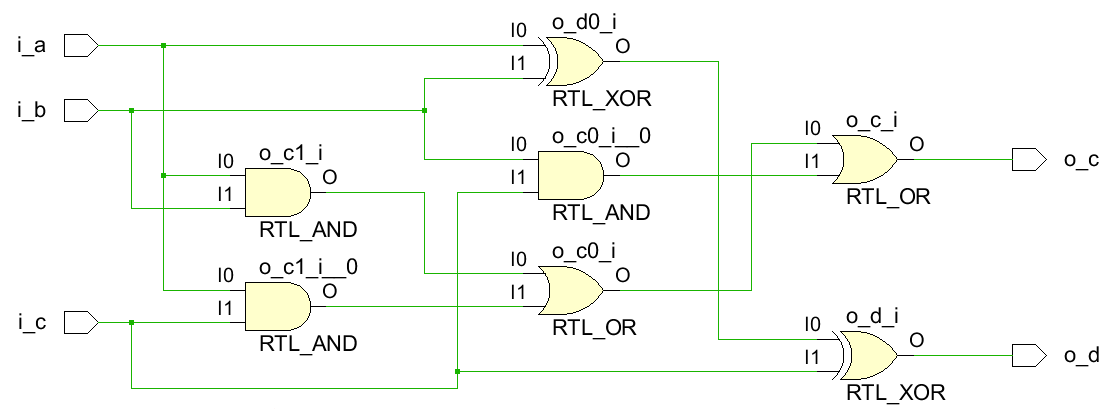
\includegraphics[width=0.9\linewidth]{rtmq/adder_case1}}
    \subcaptionbox{第二种加法器实现情况,对应公式\eqref{eq:adder2}}{
    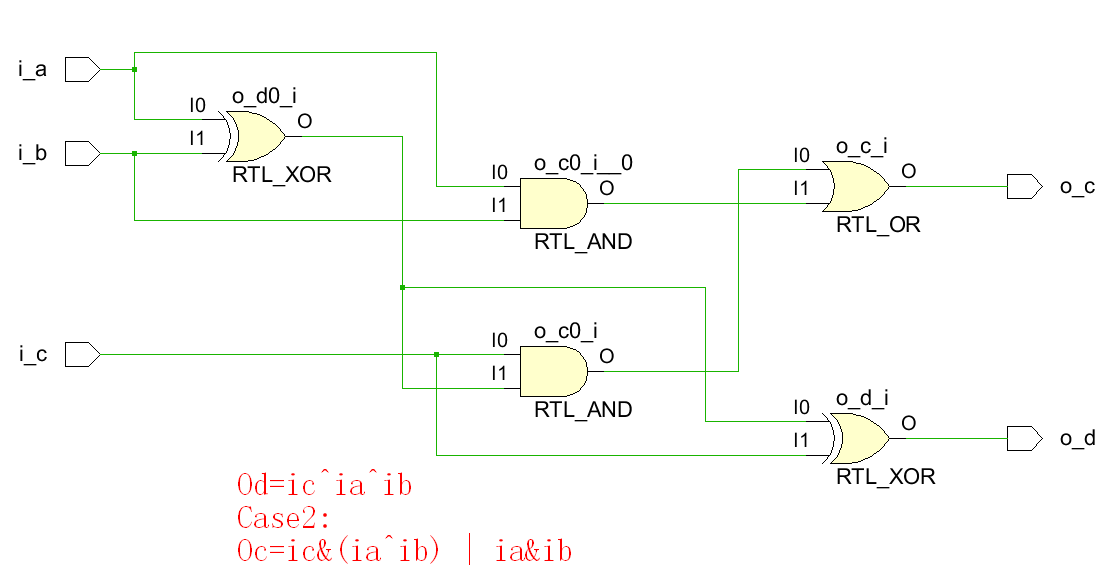
\includegraphics[width=0.9\linewidth]{rtmq/adder_case2}}
    \subcaptionbox{第三种加法器实现情况,对应公式\eqref{eq:adder3}}{
    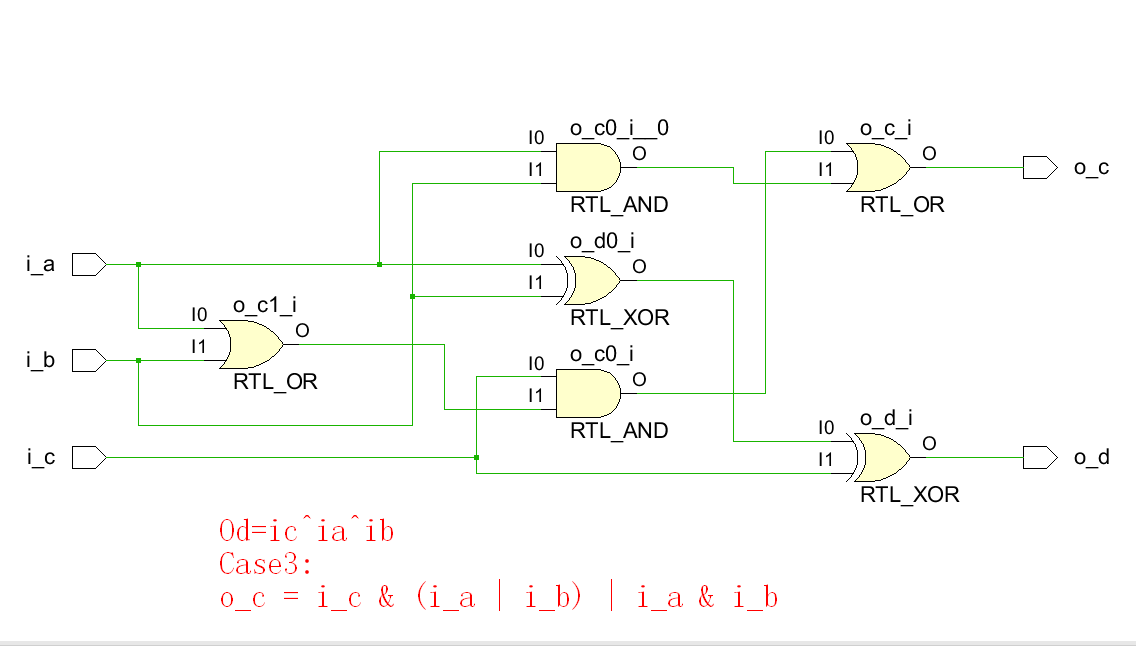
\includegraphics[width=0.9\linewidth]{rtmq/adder_case3}}
\end{figure}

三种串行进位加法器实现的结构图如图\ref{fig:carry_ripple_adder}所示。从结果可以看到,第一种写法用了7个元件,输入到输出需要三级门电路得到结果;第二种写法用了5个器件,输入到输出需要三级门电路得到结果;第三种写法用了6个元件,输入到输出需要三级门电路得到结果;从器件数量角度优选地应该使用第二种写法,具体还取决于系统可用的元器件情况。可以看出当前位对下一位的数据和进位逻辑如下:

\begin{align}
    d_i =& a_i\oplus b_i \oplus c_i\\
    c_{i+1}=& a_i \cdot b_i +(a_i \oplus b_i)\cdot c_i = G_i + (P_i)\cdot c_i
\end{align}

其中$G_i=a_i \cdot b_i$是生成信号,$P_i=a_i \oplus b_i$是传播信号。如果想要消除进位依赖,那么进位$c_{i+1}$的表达式就不能有$c_i, c_{i-1}, \dots, c_i$项,$c_0$项为初始赋予不需要替换。这里考虑四位超前进位加法器设计如下:

\begin{align}
    c_0 &= c_0\\
    c_1 &= G_0 + P_0 c_0\\
    c_2 &= G_1 + P_1 c_1 = G_1+P_1 (G_0+P_0 c_0 )=G_1+P_1 G_0+P_1 P_0 c_0\\
    c_3 &=G_2+P_2 c_2=G_2+P_2 (G_1+P_1 G_0+P_1 P_0 c_0 )\\
    &=G_3+P_3 G_2+P_3 P_2 G_1+P_3 P_2 P_1 P_0 c_0\\
    c_5 &=G_4+P_4 c_4=G_4+P_4 (G_3+P_3 G_2+P_3 P_2 G_1+P_3 P_2 P_1 P_0 c_0 )\\
    \dots\\
    c_{i+1} &=G_i+P_i G_{i-1}+P_i P_{i-1} G_{i-2}+ \dots +\prod_0^i P_j \cdot c_0
\end{align}

从中可见,对于第$i+1$位进位的计算$P_i$要参加$i+1$组计算。超前进位加法器的FPGA实现结构图如图\ref{fig:ahead_adder_4bits}所示。

\begin{figure}
    \centering
    \caption[4位超前进位加法器的FPGA实现结构图]{4位超前进位加法器的FPGA实现结构图(Vivado)\label{fig:ahead_adder_4bits}}
    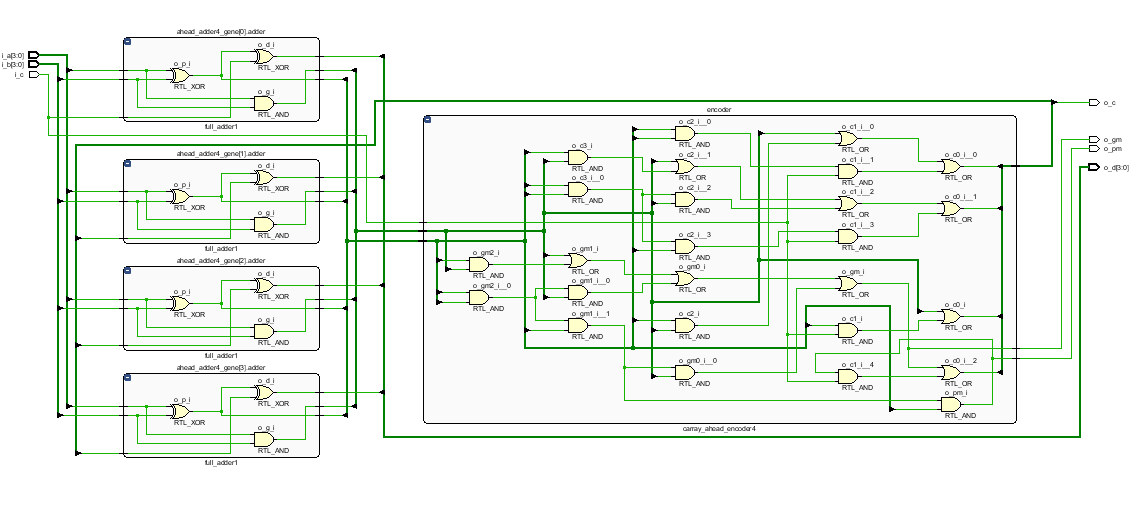
\includegraphics[width=1.0\linewidth]{rtmq/ahead_adder_4bits}
\end{figure}

按照上述规律进行拓展,可以依次得到需求位数的超前进位加法器,比如8位(附录图\ref{fig:ahead_adder_8bits})、16位(附录图\ref{fig:ahead_adder_16bits})、32位(图\ref{fig:ahead_adder_32bits})等。值得注意的是,理论上使用超前进位方式可以实现任意位数的加法器,并且实现的加法器只需要两级流水线就可以得到最终结果。不过实际上高速数字电路的延时不仅有流水线延时,还有器件延时。可以看到超前进位加法器从4位(图\ref{fig:ahead_adder_4bits})到32位(图\ref{fig:ahead_adder_32bits}),在超前进位计算的逻辑有了相当程度的复杂化了。受到器件压时延的限制,我们无法超前计算无限位数的超前进位$c_{\infty}$。

\begin{figure}
    \centering
    \caption[32位超前进位加法器的FPGA实现结构图]{32位超前进位加法器的FPGA实现结构图(Vivado)\label{fig:ahead_adder_32bits}}
    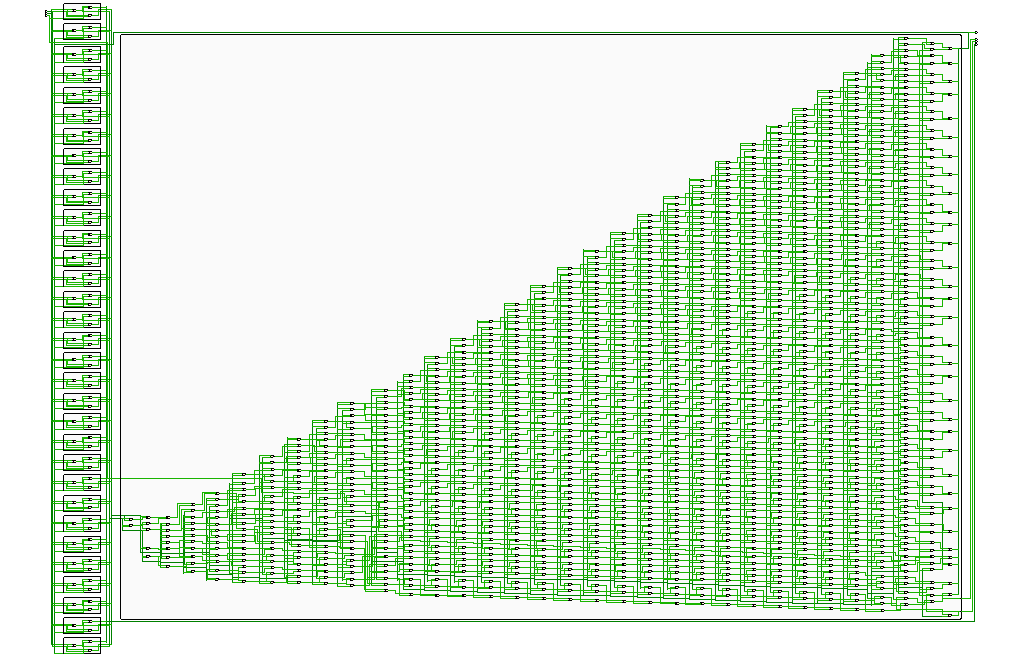
\includegraphics[width=1.0\linewidth]{rtmq/ahead_adder_32bits}
\end{figure}
\begin{figure}
    \centering
    \caption[用两个32位超前进位加法器拓展为一个64位加法器]{用两个32位超前进位加法器拓展为一个64位加法器(Vivado)\label{fig:adder_64bits}}
    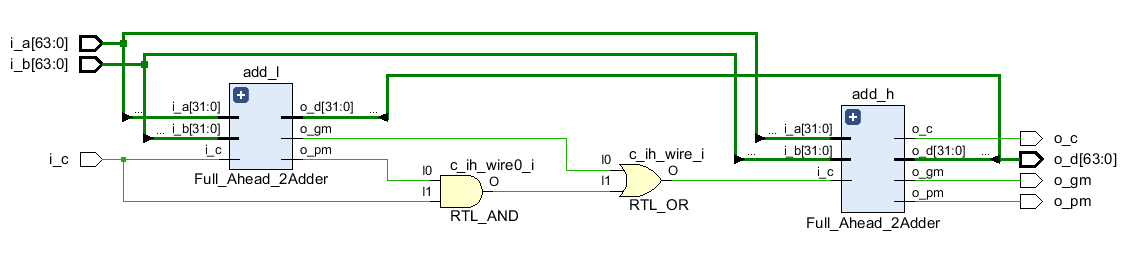
\includegraphics[width=1.0\linewidth]{rtmq/adder_64bits}
\end{figure}

一般情况下32位加法器就足够用了,比如RTMQ系统就是采用32位运算的。如果需要更高位数的加法器可以继续向上拓展,也可以考虑用串行进位加法器的思想对超前进位加法器进行拓展。

如图\ref{fig:adder_64bits}所示,这里用了两个32位加法器添加了一级流水线,拓展为了一个64位的加法器。用这种方式可以满足一些特殊的更高位数加法器的实现。不过,在流水线时延上要做出一点妥协。







\newpage
\section[基于FPGA的数字Booth乘法器]{基于FPGA的数字Booth乘法器\label{section:booth_multiplier}}
% \textcolor{red}{
% 1. 介绍数字Booth乘法器功能、逻辑图、Vivado中的实现、优势;}
布斯(Booth)乘法器是一种对乘数进行重新编码,以减少乘法运算中所需的加法次数的乘法器。它由布斯夫妇于 1950 年发明,因硬件实现简单、所需硅片面积较小、能够显著提高乘法运算速度而被广泛采用。

Booth乘法器通过相加和相减的操作计算补码数据的乘积。该算法对乘数从低位开始判断,根据后两个数据位的情况决定进行加法、减法还是仅仅进行移位操作。
在计算两个补码相乘时,会将上一轮编码产生的进位与当前轮编码进行相加,然后再进行移位操作。通过这种方式,布斯乘法器可以减少乘法运算中所需的加法次数,从而提高计算速度。

Booth乘法器在数字信号处理、计算机算术、密码学等领域中具有广泛的应用\cite[]{Jigjidsuren_Badarch_Sukhbaatar_Namsrai_2021}。在RTMQ系统中有关的乘法运算基本都是以Booth乘法器来实现的。下面将介绍它的原理和实现。

\subsection[乘法基本]{乘法基本}
不采用任何优化算法的乘法过程可以用列竖式乘法来表示。从乘数的低位开始,每次取一位与被乘数相乘,乘积作为部分积(Partial Product, PP)暂存。乘数的全部有效位乘完后,再将所有部分积(PP0-PPx)按照对应乘数位的相应权重错位相加,得到最后的乘积。如图\ref{fig:multiple_process}所示,左图和右图分别展示了十进制数和二进制数的无优化算法乘法过程,可见二进制乘法和十进制乘法本质上并无差别。

\begin{figure}
    \centering
    \caption[十进制数和二进制数的无优化算法乘法过程]{十进制数和二进制数的无优化算法乘法过程\label{fig:multiple_process}}
    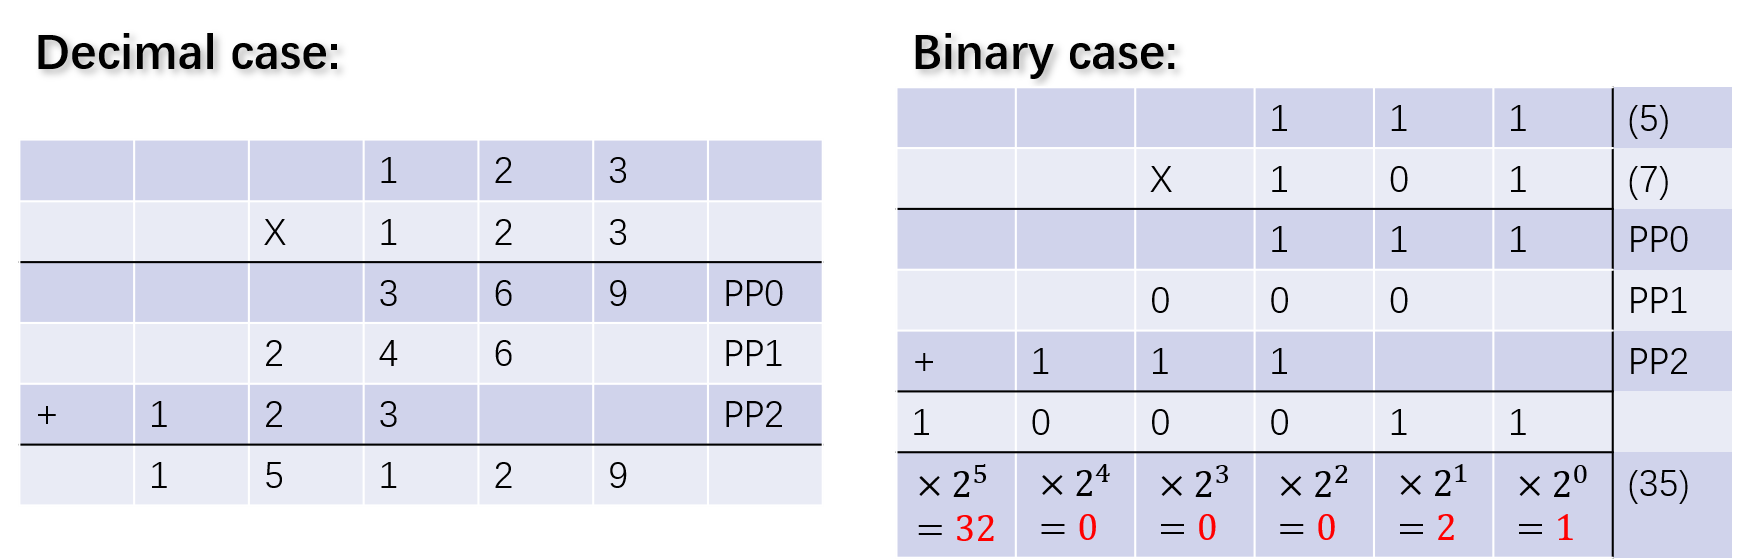
\includegraphics[width=1.0\linewidth]{rtmq/multiple_process}
\end{figure}

如果将乘法过程表示成通式,比如4位乘法器,如图\ref{fig:multiple_process_general}所示。这样原始的乘法在设计上是可以实现的,但在工程应用上几乎不会采用,在时延与面积上都需要优化。一个$n_1=n_2=N$位的乘法运算,需要产生$N$个部分积,并对它们进行全加处理,位宽越大,部分积个数越多,需要的加法器也越多,加法器延时也越大,这对高速芯片来说是很不有好的。实际上乘法过程拆解开来就是获得部分积和处理部分积相加的过程。由于在二进制中获得部分积的过程可以通过简单的移位来实现,因此针对乘法运算的优化,主要就集中在两个方面:一是减少部分积的个数,二是减少加法器带来的延时。而Booth编码的方式就是从减少部分积的个数的角度来优化乘法运算的,下一小节将介绍Booth编码相关概念。

\begin{figure}
    \centering
    \caption[4位乘法过程通式]{4位乘法过程通式\label{fig:multiple_process_general}}
    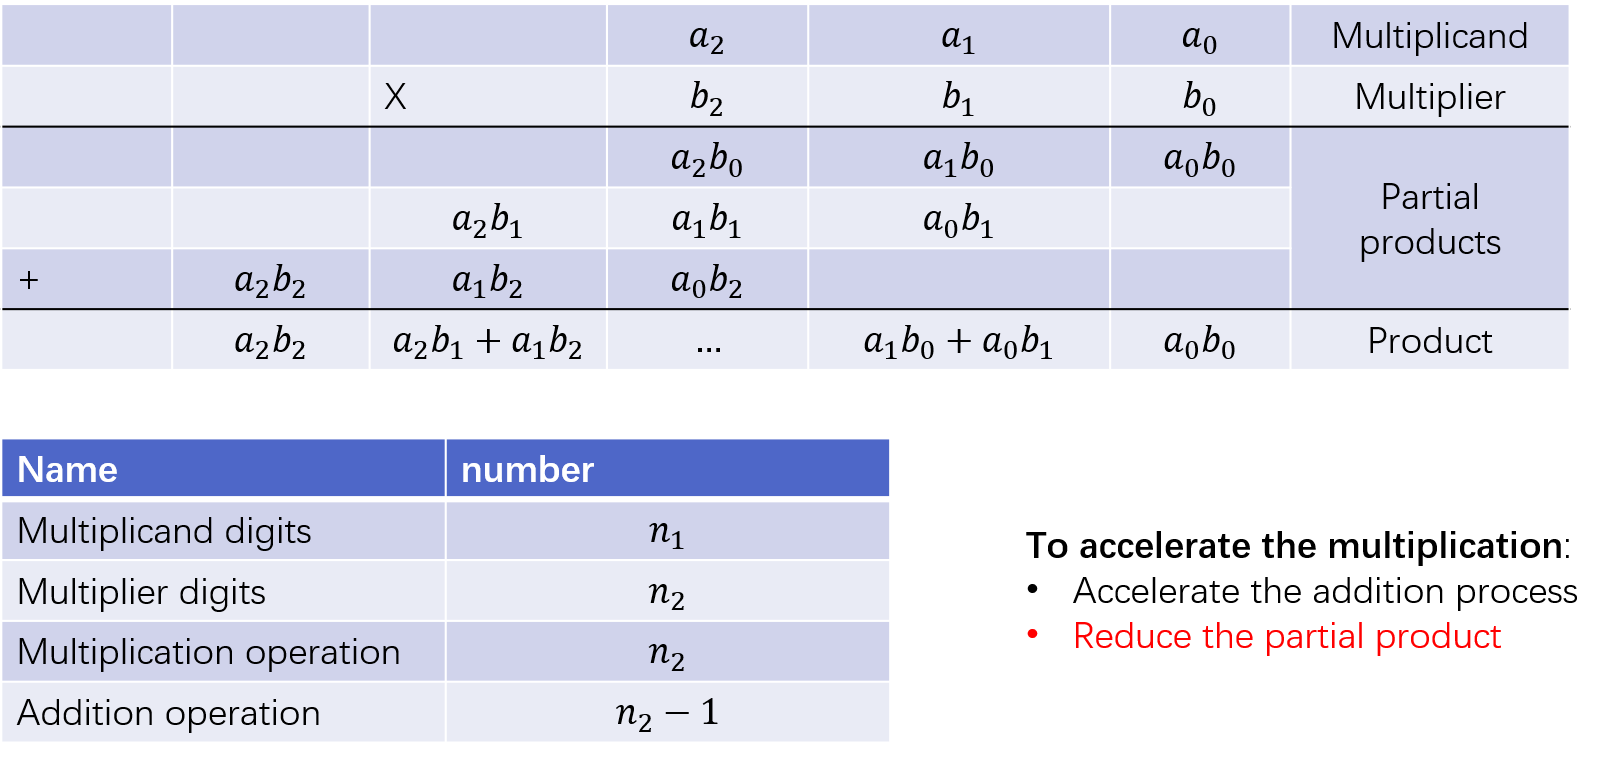
\includegraphics[width=1.0\linewidth]{rtmq/multiple_process_general}
\end{figure}

\subsection[改进的Booth编码]{改进的Booth编码}

任意$n$比特的有符号数可以表示为:
\begin{align}
    y=&-2^{n-1} y_{n-1}+2^{n-2} y_{n-2}+\\
    &…+2^2 y_2+2^1 y_1+2^0 y_0+y_{-1}\label{eq:binary_number_expression}
\end{align}

其中$-2^(n-1) y_(n-1)$是符号,$y_(-1)=0$是添加的辅助比特。公式\ref{eq:binary_number_expression}可以被进一步变形为:

\begin{align}
    y=&-2^{n-1} y_{n-1}+(2^{n-2} y_{n-2}+2^{n-2} y_{n-2} )-2^{n-2} y_{n-2}+…+(2^2 y_2\\
    &+2^2 y_2 )-2^2 y_2+(2^1 y_1+2^1 y_1 )-2^1 y_1+(2^0 y_0+2^0 y_0 )-2^0 y_0+y_{-1}\\
    =&-2^{n-1} y_{n-1}+(2^{n-1} y_{n-2} )-2^{n-2} y_{n-2}+\\
    &…+(2^3 y_2 )−2^2 y_2+(2^2 y_1 )-2^1 y_1+(2^1 y_0 )-2^0 y_0+y_{-1}\\
    =&2^{n-1} (-y_{n-1}+y_{n-2} )+2^{n-2} (-y_{n-2}+y_{n-3} )+\\
    &…+2^1 (-y_1+y_0 )+2^0 (-y_0+y_{-1})\label{eq:binary_number_expression1}
\end{align}

通过公式\eqref{eq:binary_number_expression1}可以发现,多项表达式的项数变成了原来的一半。原二进制数从LSB(最低位)开始,以三位为一组(第一组最低位需补一个附加位即$y[-1]$,附加值为$0$),相邻组之间重叠一位(低位组的最高位与高位组的最低位重叠),构成新的多项式因子,这就是\emph{改进的布斯编码}方式。

两个二进制数乘,如果对乘数进行公式\eqref{eq:binary_number_expression1}所示的改进型布斯编码,则得出的部分积个数相较直接相乘可以减半。比如,两个32位数相乘,不做布斯编码直接相乘,则有32个部分积需要累加,而采用 式3 的编码方式对其中一个因数进行变换后,将只有16个部分积需要累加。

由公式\eqref{eq:binary_number_expression1}可知,组成多项式因子的每连续三位之间的关系是完全相同的,二进制中每一位的数值非0即1,由此可以列出相邻三位所有取值组合下,其对应多项式因子的值。设某乘法运算中,被乘数为$X$,乘数为$Y$,$Y_{i+1},\ Y_{2i},\ Y_{2i-1}$分别为$Y$的连续三位,其中$i$为自然数$N$,$PP_i$为$i$不同取值下对应的部分积,对$Y$进行改进的布斯变换后再与$X$相乘,则可以有如表\ref{tb:booth_lookup_table}推算关系。

\begin{table}
    \centering
    \caption[基4布斯编码查找表]{基4布斯编码查找表\label{tb:booth_lookup_table}}
    \begin{tabular}{C{2cm}C{2cm}C{2cm}|C{2cm}}
        \toprule 
        \multicolumn{3}{c}{\textbf{Input}} &\textbf{Output}\\
        \toprule
        $Y_{2i+1}$ & $Y_{2i}$ & $Y_{2i-1}$ & $PP_i$\\
        \hline
        0 & 0 & 0 & 0 \\
        1 & 0 & 0 & X\\
        0 & 0 & 1 & X\\
        1 & 0 & 1 & 2X\\
        0 & 1 & 0 & -2X\\
        1 & 1 & 0 & -X\\
        0 & 1 & 1 & -X\\
        1 & 1 & 1 & 0\\
        \bottomrule
    \end{tabular}
\end{table}

由此可见,根据乘数每连续三位的值,可以快速推算出其对应的部分积。且在二进制中,乘2操作可以通过左移一位来实现,不需要复杂的计算,电路实现非常简单,通过此方法,解决了硬件乘法优化的第一个方面,简化和减少部分积的生成。作为改进型布斯编码中最基础的一种,它被称之为基4布斯编码。基4编码相当于每次用乘数的两位与被乘数相乘产生部分积,从而使部分积个数减少一半,也可以看成是将乘数转化为4进制表达,故称为基4(Radix-4 Booth Encoding)。采用基4布斯编码的乘法相较于传统乘法运算,优化效果已经很明显且易于实现,可以满足大部分应用要求,32位乘法器,甚至64位乘法器都可以采用,是比较常用的一种方式。当然,更高阶的布斯编码可以更大程度地减少部分积个数,但因其部分积产生逻辑无法单纯通过移位实现,需要引入加法器等其它运算部件,从这方面来看又削弱了优化效果,需要综合考量选择。

\subsection[进位保留加法器与3-2压缩、4-2压缩]{进位保留加法器与3-2压缩、4-2压缩}
布斯编码解决了乘法优化的第一个方面,通过减少部分积个数从而减少累加器个数,但累加器本身的进位传递延时对电路性能依然存在非常大的影响,所以优化的第二个方面,就是改进部分积累加结构,提升累加性能。如果采用部分积直接相加的方式,因为全加器进位的关系,当前bit的相加结果依赖于它前一bit的进位输出,整个计算过程相当于串行化,位宽越大,延时越大,所以优化的关键就是消除进位链,使运算并行化。

进位保留加法器(Carry Save Adder, CSA)是比较常用的一种优化方式,CSA实际上就是一位全加器,其逻辑表达示如下:


进位保留加法器编码相当于一次接受三个输入,产生两个输出,因此也称为3-2计数器或3-2压缩(3-2编码)。如图\ref{fig:carray_save_adder_clock}所示,运用到乘法器中,通过对若干个部分积按每3个为一组进行CSA计算,然后用同样的方法运用到每级CSA产生的输出上,直到最后一级CSA的两个输出,再用全加器得到最后的部分积累加结果。
\begin{figure}
    \centering
    \caption[进位保留加法器编码(3-2编码)]{进位保留加法器编码(3-2编码)\label{fig:carray_save_adder_clock}}
    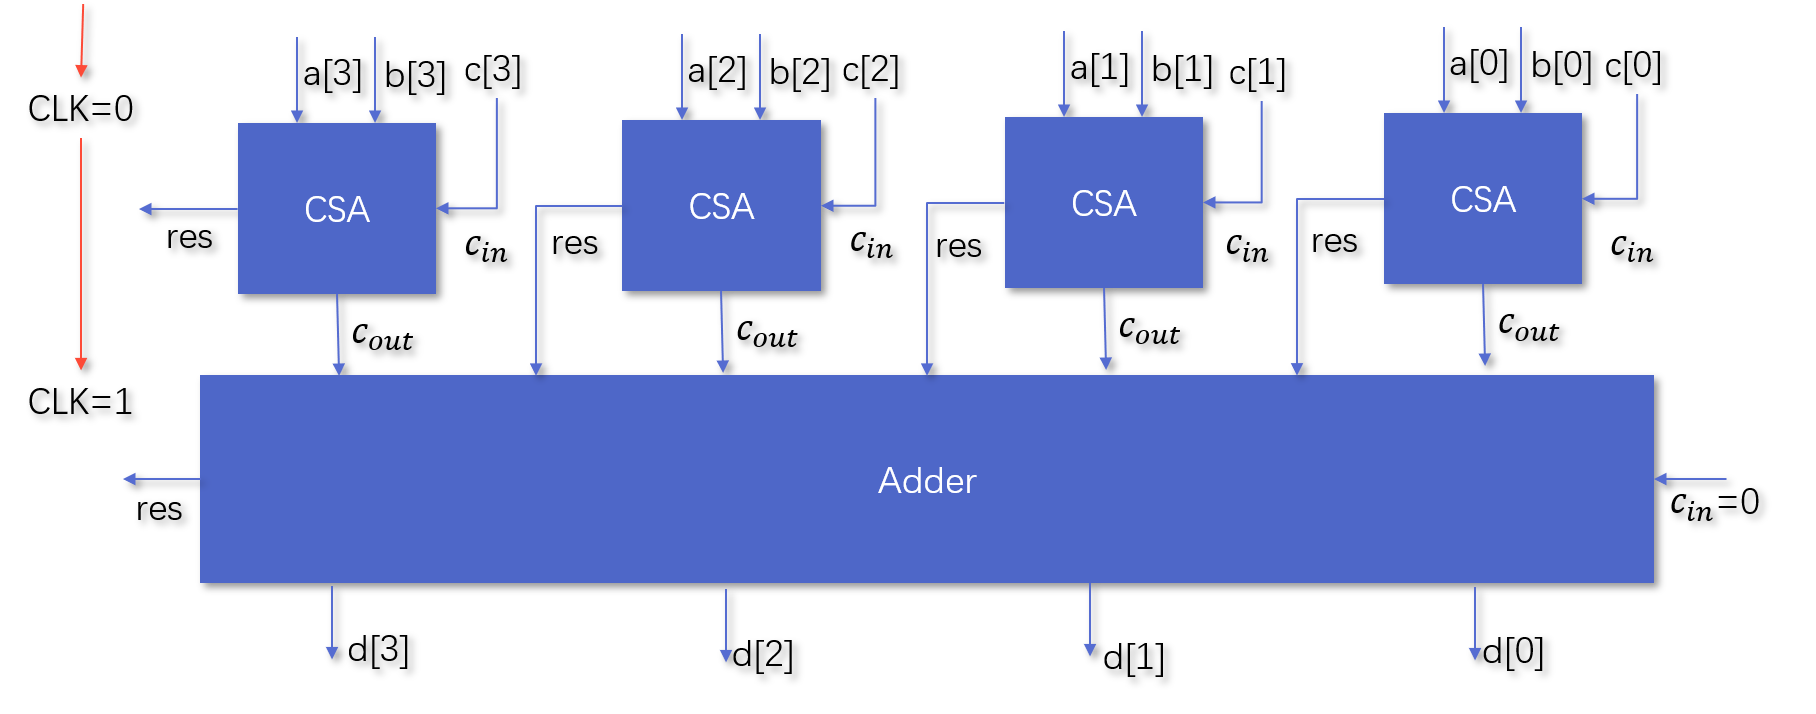
\includegraphics[width=1.0\linewidth]{rtmq/carray_save_adder_clock}
\end{figure}

相较于3-2压缩,还有一种压缩率更高的方式叫4-2压缩(编码),或称为5-3计数器。顾名思义,就是有5个输入端,产生3个输出,运用到加法上,可以实现同时计算四个加数,生成对应的结果与进位值。设5-3计数器的5个输入分别为$I[0], I[1], I[2], I[3], C_i$,3个输出端分别为$ D, C, C_o$,则它们之间满足如下代数关系:
\begin{align}
    D+C\times 2+C_o\times 2=I_0+I_1+I_2+I_3+C_i\label{eq:encoder_5to3}
\end{align}
根据公式\eqref{eq:encoder_5to3},可以推算出相应的真值表如表\ref{tb:encoder_5to3}所示。
\begin{table}
    \centering
    \caption[4-2压缩器真值表]{4-2压缩器真值表\label{tb:encoder_5to3}}
    \begin{tabular}{C{1.5cm}|C{4cm}|C{1.5cm}C{1.5cm}C{1.5cm}}
        \toprule 
        \multicolumn{2}{c}{\textbf{Input}} &\multicolumn{3}{c}{\textbf{Output}}\\
        \toprule
        $C_i$ & $I_0+I_1+I_2+I_3$ & $C_0$ & $C$ & $D$\\
        \midrule
        \multirow{5}{3cm}{0} & 0 & 0 & 0 & 0 \\
        & 1 & 0   & 0     & 1 \\
        & 2 & 0/1 & 1/0   & 0 \\
        & 3 & 0/1 & 1/0   & 1 \\
        & 4 & 1   & 1     & 0\\
        \hline
        \multirow{5}{3cm}{1} & 0 & 0 & 0 & 1\\
        & 1 & 0/1 & 1/0   & 0 \\
        & 2 & 0/1 & 1/0   & 1 \\
        & 3 & 1   & 1     & 0 \\
        & 4 & 1   & 1     & 1 \\
        \bottomrule
    \end{tabular}
\end{table}

输出与输入之间的逻辑经化简最后可表达示为:
\begin{align}
    D=&I_0\oplus I_1\oplus I_2\oplus I_3 \oplus C_i\\
    C=&((I_0\oplus I_1\oplus I_2\oplus I_3)\cdot C_i)\\
    &+\neg ((I_0\oplus I_1\oplus I_2\oplus I_3)+\neg((I_0\cdot I_1)+(I_2\cdot I_3)))\\
    C_o=&(I_0+I_1)\cdot(I_2+I_3)
\end{align}
\subsection[Booth乘法器的硬件实现]{Booth乘法器的硬件实现}
下面以一个$8\times 8$的乘法器为例,介绍运用上述介绍设计和实现Booth乘法器的方法,更大位宽的乘法器可以通过类似的方法拓展得到。

前面对算法原理的论述中,没有提及有符号数和无符号数,但在设计的时候,则需要考虑有符号数与无符号数的区别。实际上布斯编码是带符号位的,也就是它的编码方式是建立在有符号数基础之上,从多项式1的最高次项也可以看出来。所以,采用布斯编码的乘法器是一种有符号数乘法器,或者说补码乘法器(原码与补码的关系不在此文讨论范围)。为了使乘法器能够兼容无符号数计数,可以对乘数扩展一位符号位,当计算无符号数时,该位为0;当计算有符号数时,该位等于扩展前的符号位。如此会导致增加一个部分积,但带来的便利是对两种不同性质的数可以采用完全一样的计算方式,下面的设计实例遵循此方式进行。

设$A[8:0], B[8:0]$分别为乘法器的两个输入,以$A$为被乘数,$B$为乘数。$A[8]$和$B[8]$为兼容无符号数扩展的符号位。

首先,根据前文内容,对乘数B以基4的方式进行改进型布斯编码,即从LSB开始,以每3bit为一组进行分组,每相邻两组之间的最高位与最低位重合(红色位),LSB的右边还需增加一个附加位,定义为$B[-1]$,值为零。如图\ref{fig:booth_multiplier_8bits_basic1}所示。

\begin{figure}
    \centering
    \caption[8位Booth乘法器编码表]{8位Booth乘法器编码表\label{fig:booth_multiplier_8bits_basic1}}
    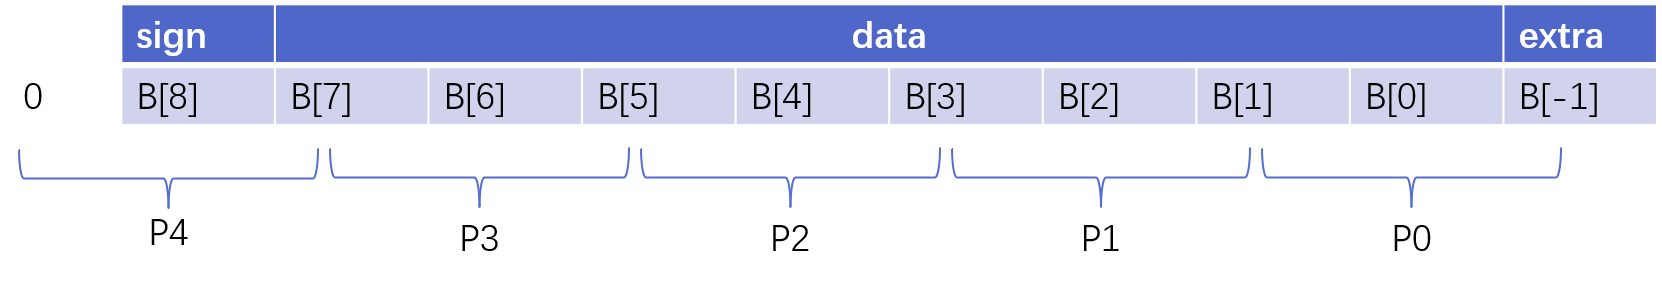
\includegraphics[width=1.0\linewidth]{rtmq/booth_multiplier_8bits_basic1}
\end{figure}


$B[1:-1]$为第1组,$B[3:1]$为第2组,$B[5:3]$为第3组,依此类推,一共可划分为5组。其中第5组因为不够3个bit,故在最高位再扩展一位符号位,符号位的扩展并不会改变补码数据的值。根据每组的值和表\ref{tb:booth_lookup_table}的查找关系,可得出对应的部分积,一共产生5个部分积,定义为PP0-PP4。相邻两组部分积之间权重相差4倍,相当于二进制运算中的左移两位,于是可以将部分积按对应权重排列为如图\ref{fig:booth_multiplier_8bits_basic0}形式。
\begin{figure}
    \centering
    \caption[8位Booth乘法器部分积排列表]{8位Booth乘法器部分积排列表\label{fig:booth_multiplier_8bits_basic0}}
    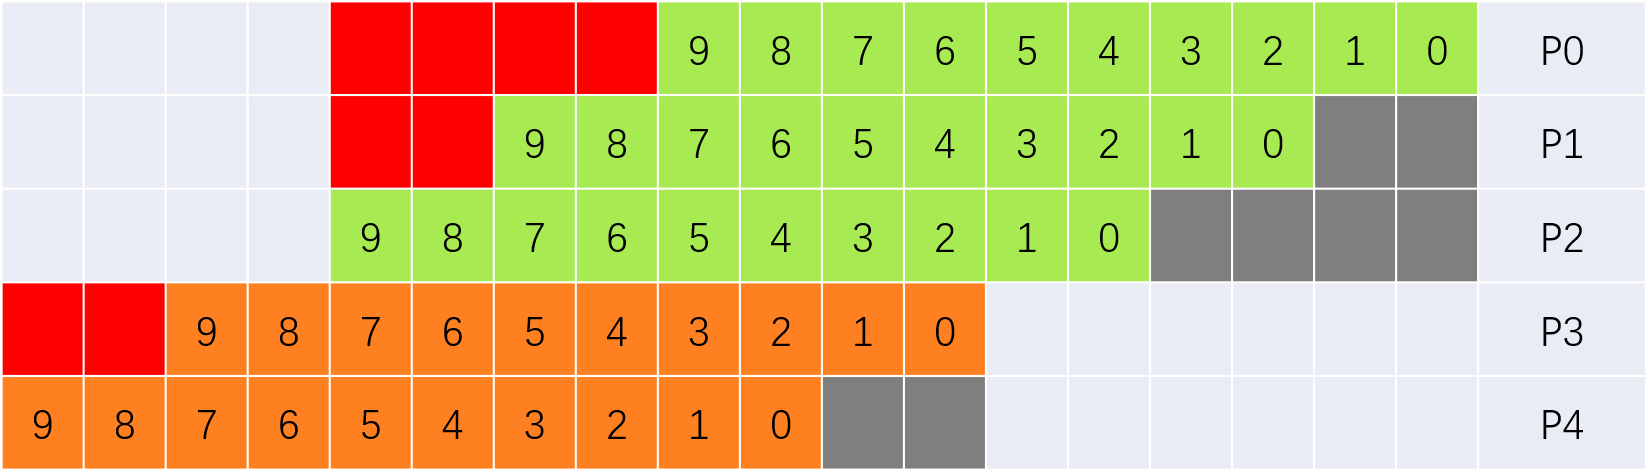
\includegraphics[width=1.0\linewidth]{rtmq/booth_multiplier_8bits_basic0}
\end{figure}

\subsection[3-2压缩器组建加法树]{3-2压缩器组建加法树}
部分积生成后,即可组建加法树。加法树的构成采用3-2压缩方式,8位Booth乘法器的编码表和加法树如图\ref{fig:booth_multiplier_8bits_basic}所示。

% 8位Booth乘法器的编码表和编程设计图如图\ref{fig:booth_multiplier_8bits_basic}所示。
\begin{figure}
    \centering
    \caption[8位Booth乘法器加法树的构建]{8位Booth乘法器加法树的构建\label{fig:booth_multiplier_8bits_basic}}
    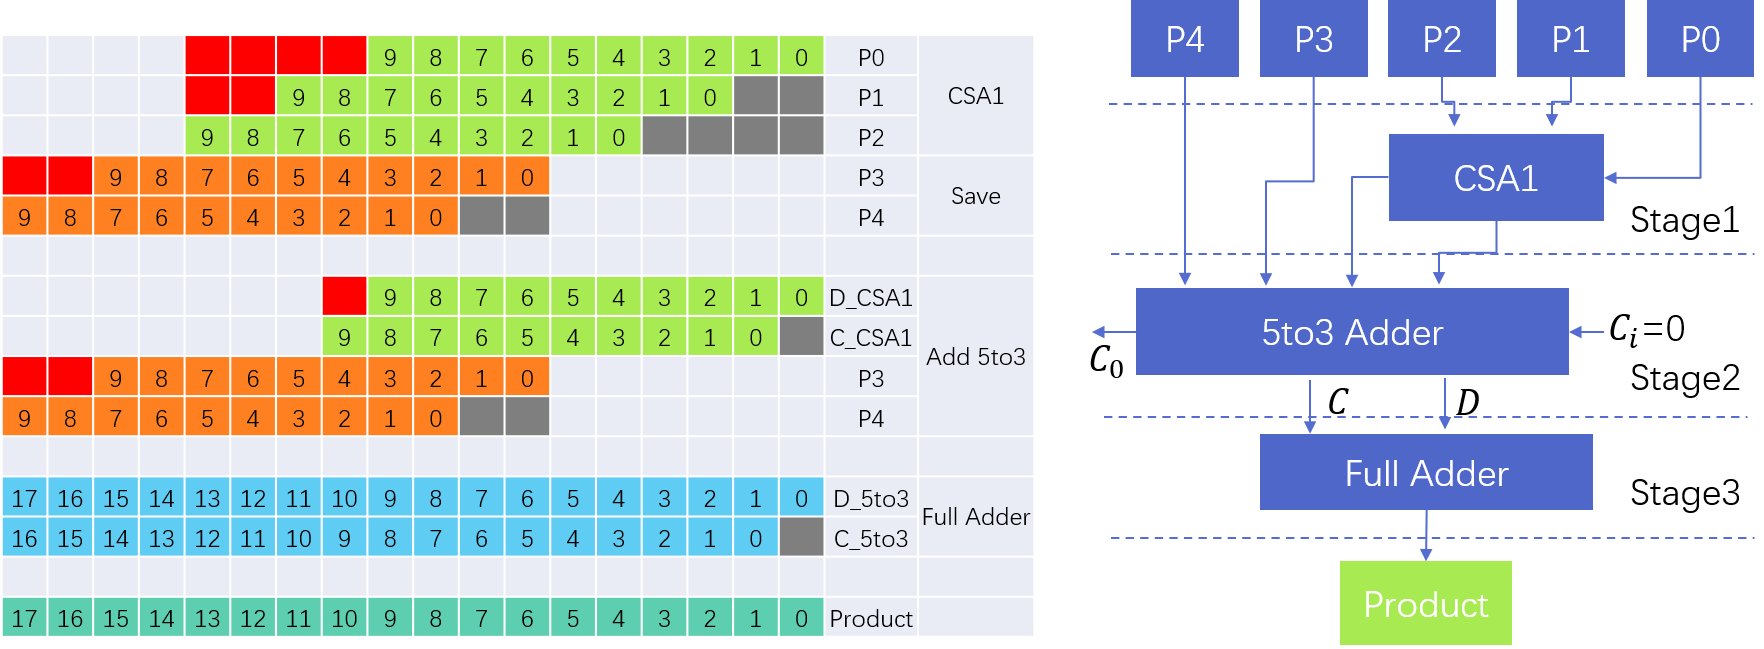
\includegraphics[width=1.0\linewidth]{rtmq/booth_multiplier_8bits_basic}
\end{figure}

5个部分积分别为PP0-PP4,从PP0开始,每三个为一组进行3-2压缩,使用一个3-2压缩器。在第一级中PP0-PP2使用一个3-2加法器,由于P3和P4不足三个输入,在第一级进行保留;第二级中的输入有4个,正好可以采用一个4-2编码器;在第三级中可以直接采用全加器计算得到最终结果。在每个3-2压缩或者4-2压缩的过程中,相邻部分积由于偏移造成的输入不足时,低位补0(图表中灰色填充部分),高位补符号位(图表中红色填充部分)。8位乘法器的正常积结果为16位,因此超过16位的部分可以直接舍弃不参与运算。

综上例子中的$8\times 8$Booth乘法器采用了一个3-2编码器、一个4-2编码器和一个16位全加器,经过3级流水线计算得到最终积。加法树的拓扑可以有很多选择,比如也可以仅采用3-2编码器或者仅采用4-2编码器,一般来说优化的方向是编码级数尽量少、器件尽量少,具体可以根据实际应用进行取舍。

从上面的叙述中可以看出,Booth乘法器的实现重点是要获得一个编码和加法树表,根据加法树表可以绘制出相应的加法树,并进一步在代码中实现。
16位Booth乘法器的编程设计图如图\ref{fig:booth_multiplier_16bits_basic}所示。相应的结构示意图如图\ref{fig:booth_multiplier_16bits_basic_s}所示。
\begin{figure}
    \centering
    \caption[16位Booth乘法器编码和加法树表]{16位Booth乘法器编码和加法树表\label{fig:booth_multiplier_16bits_basic}}
    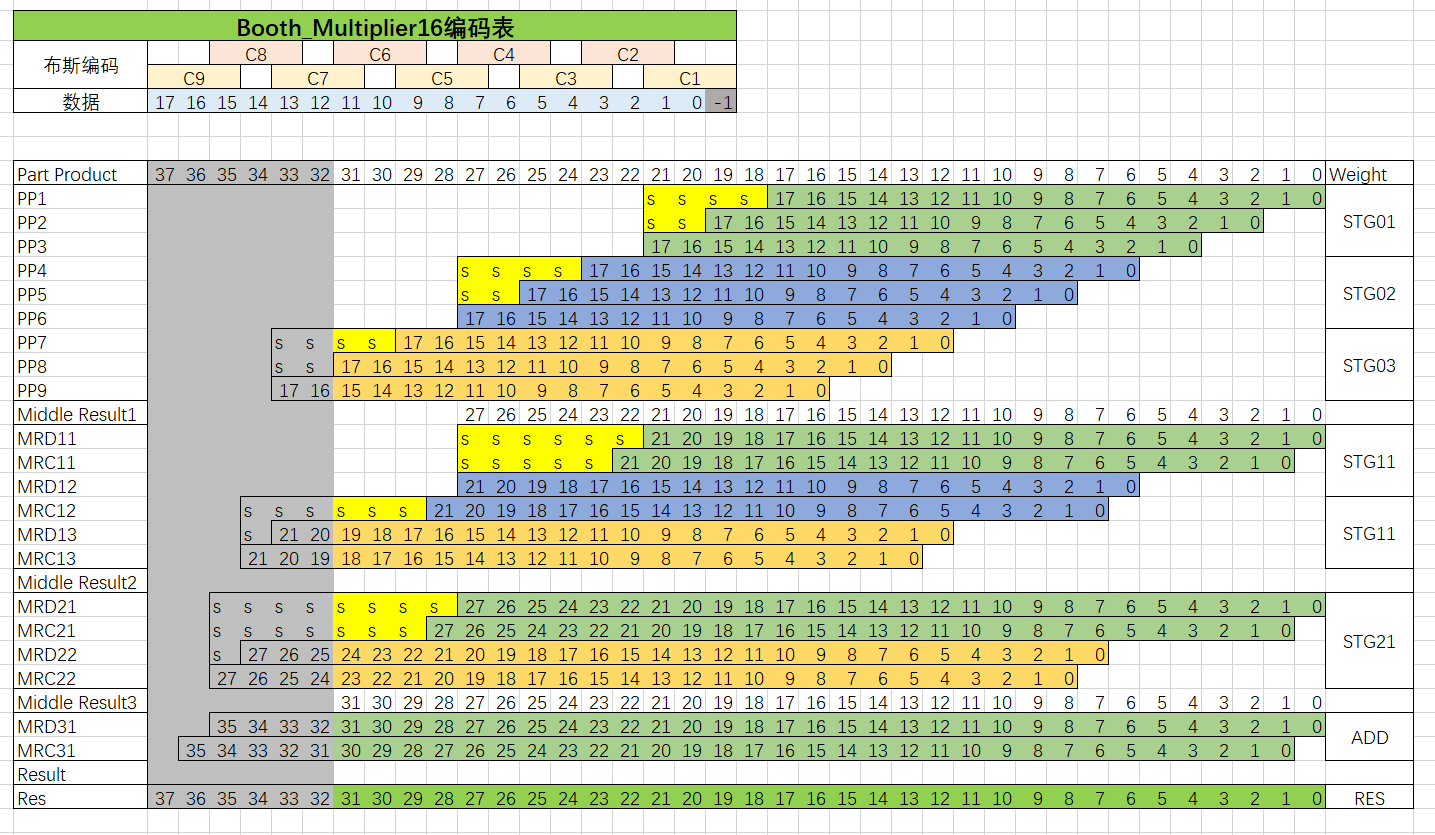
\includegraphics[width=1.0\linewidth]{rtmq/booth_multiplier_16bits_basic}
\end{figure}

\begin{figure}
    \centering
    \caption[16位Booth乘法器结构示意图]{16位Booth乘法器结构示意图\label{fig:booth_multiplier_16bits_basic_s}}
    \includesvg[width=1.0\linewidth]{rtmq/booth_multiplier_16bits_basic_s}
\end{figure}

上述实现的16位Booth乘法器已经可以满足RTMQ系统的基本使用需求了。更高位数的Booth乘法器实现可以依据上述规律进行设计开发。作为扩展,附录图\ref{fig:booth_multiplier_16bits_basic}给出了32位Booth乘法器的编码表和加法树表。









\newpage
\section[基于FPGA的数字PID]{基于FPGA的数字PID\label{section:digital_pid}}
% \textcolor{red}{
% 1. 介绍数字PID功能、逻辑图、Vivado中的实现、优势;}
\subsection[数字PID]{数字PID}
数字PID控制器是一种常用的自动控制算法,用于实现对系统的闭环控制。PID控制器通过对系统的误差进行比例(Proportional)、积分(Integral)和微分(Derivative)计算,生成控制信号来调整系统的输出,以达到期望的控制效果。在量子测控系统中很多地方都需要用到闭环控制,比如激光的功率稳定、激光的波长稳定、离子阱频率稳定等。相对于模拟PID控制器,数字PID控制器具有结构简单、易于实现、控制灵活、工作稳定等优点,是RTMQ系统中的重要组成部分。

PID 控制器的数学表达式可以表示为:
\begin{align}
    u(t)= K_p e(t) + K_i \int_{0}^{t} e(\tau) d\tau + K_d \frac{d e(t)}{dt}
\end{align}

其中,$u(t)$是控制器的输出,$e(t)$是系统的误差,$K_p$、$K_i$和$K_d$分别是比例系数、积分系数和微分系数。
 
PID控制器的实现可以分为模拟PID和数字PID两种方式。模拟PID是通过模拟电路实现的,而数字PID是通过数字计算实现的。数字PID控制器通常使用微处理器或计算机来实现,其基本结构包括采样、计算和输出三个部分。数字 PID 控制器的实现步骤如下:
\begin{itemize}
    \item 采样:对系统的输入和输出进行采样,获取当前时刻的误差值e(t);
    \item 计算:根据采样得到的误差值,按照 PID 控制器的数学表达式计算控制信号u(t);
    \item 输出:将计算得到的控制信号输出到执行机构,调整系统的输出;
\end{itemize}

在数字PID控制器的实现中,需要对积分和微分操作进行离散化处理。常用的离散化方法有矩形法和梯形法。矩形法将积分区间划分为若干个相等的子区间,每个子区间的积分值近似为矩形的面积;梯形法将积分区间划分为若干个相等的子区间,每个子区间的积分值近似为梯形的面积。这一步骤在嵌入式系统中通常使用模拟数字转换(ADC)芯片来完成。

\subsection[数字PID的增量表达式]{数字PID的增量表达式}
\begin{figure}
    \centering
    \caption[数字PID结构示意图]{数字PID结构示意图\label{fig:digital_pid_structure_16bits_s}}
    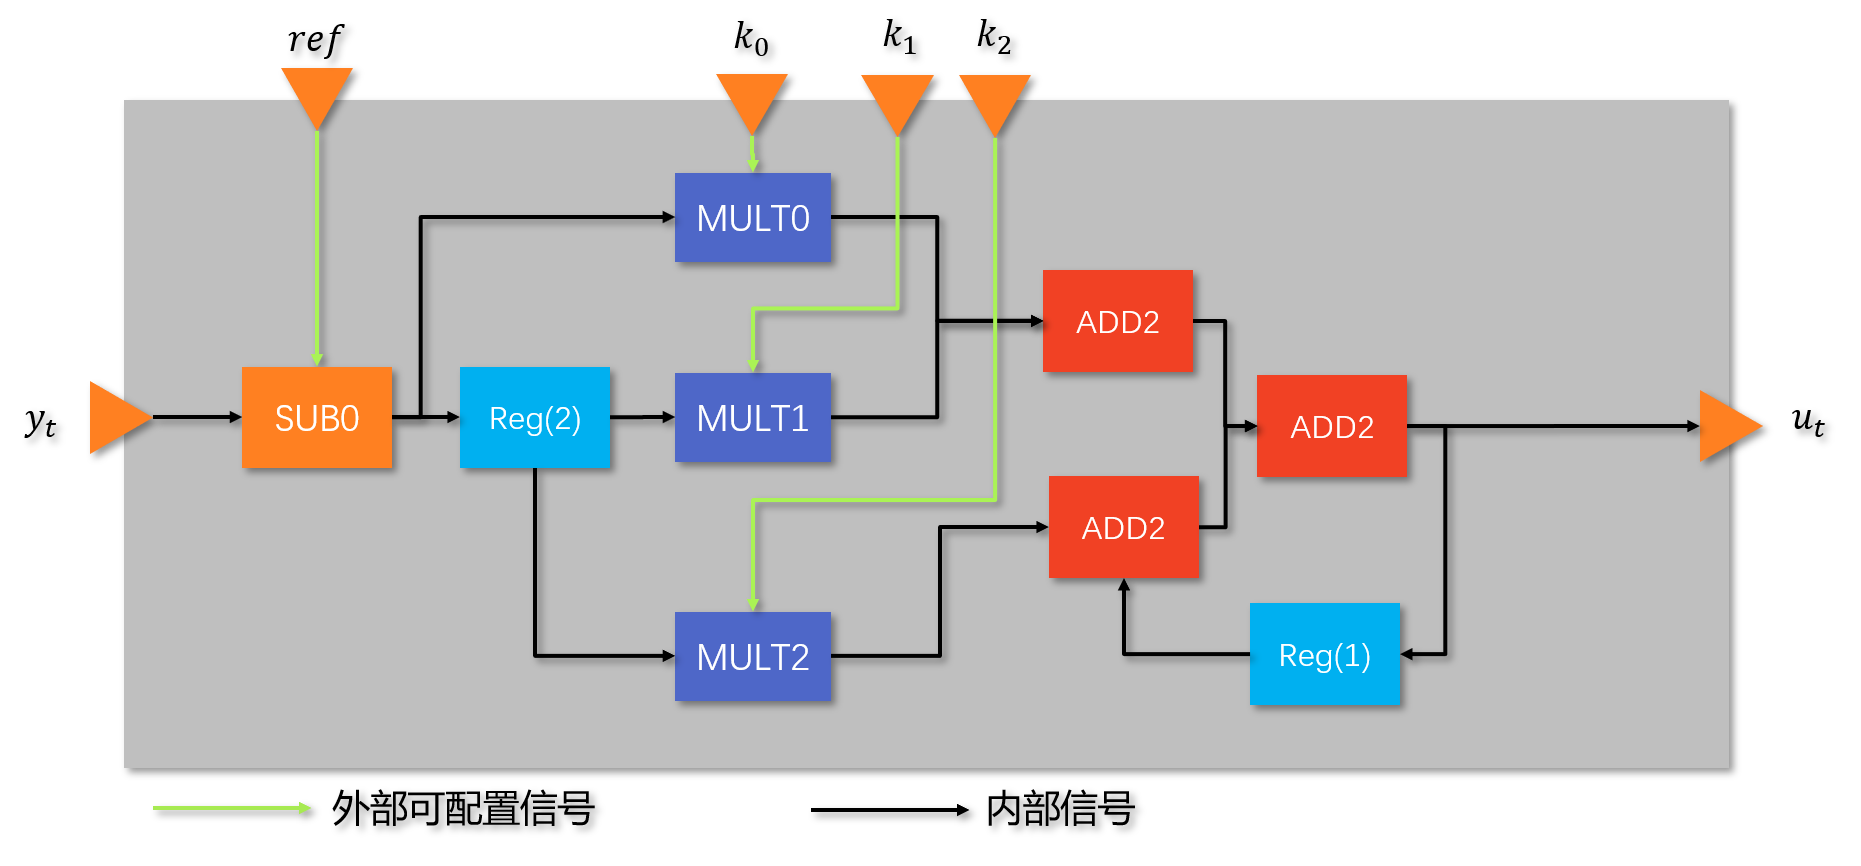
\includegraphics[width=1.0\linewidth]{rtmq/digital_pid_structure_16bits_s}
\end{figure}

离散化后的PID表达式为:
\begin{align}
    u(n)=k_p e(n)+k_i\sum_{j=-}^{n}e(j)+k_d[e(n)-e(n-1)]\\
    u(n-1)=k_p e(n-1)+k_i \sum_{j=0}^{n-1}e(j)+k_d [e(n-1)-e(n-2)]
\end{align}

由上面两式可以导出:

\begin{align}
    \Delta u(n)=&u(n)-u(n-1)\\
    =&k_0 e(n)+k_1 e(n-1)+k_2 e(n-2)
\end{align}

其中$k_0=k_p+k_i+k_d,\ k_1=-k_p-2k_d,\ k_2=k_d$,这个式子被称为PID的增量算法。采用这种形式的好处是避免了计算PID原始表达式中的无限积分项。在这种增量式的方式下,PID的控制输出可以表达为:
\begin{align}
    u(n)=u(n-1)+\Delta u(n)=u(n-1)+k_0 e(n)+k_1 e(n-1)+k_2 e(n-2)\label{eq:increment_pid}
\end{align}

按照上述式\eqref{eq:increment_pid}表示的增量式算法,数字PID实现的结构示意图如图\ref{fig:digital_pid_structure_16bits_s}所示。接口主要有参考$ref$、参数$k_0, k_1, k_2$等可配置输入,反馈信号$y_t$等系统回路输入,以及$u_t$等系统控制输出。用到的器件包括加法器/减法器(图示中红、橙色模块)、乘法器(图示中蓝色模块)、寄存器(图示中靛色模块)。

\subsection[数字PID的FPGA实现]{数字PID的硬件实现}

% 增量式PID最终在FPGA中实现的结构图如图\ref{fig:digital_pid_structure_16bits}所示。

根据图\ref{fig:digital_pid_structure_16bits_s}所示的结构,可以在FPGA中实现硬件的PID。其中涉及到的数字加法器、数字乘法器在第\ref{section:carray_lookahead_adder}节和第\ref{section:booth_multiplier}节中已经有过介绍。对于高速时序电路,在开发过程中需要注意流水线的设置和对齐,最终的实现硬件框图如图\ref{fig:digital_pid_structure_16bits}所示。
\begin{figure}
    \centering
    \caption[16位数字PID的FPGA实现结构图]{16位数字PID的FPGA实现结构图上\label{fig:digital_pid_structure_16bits}}
    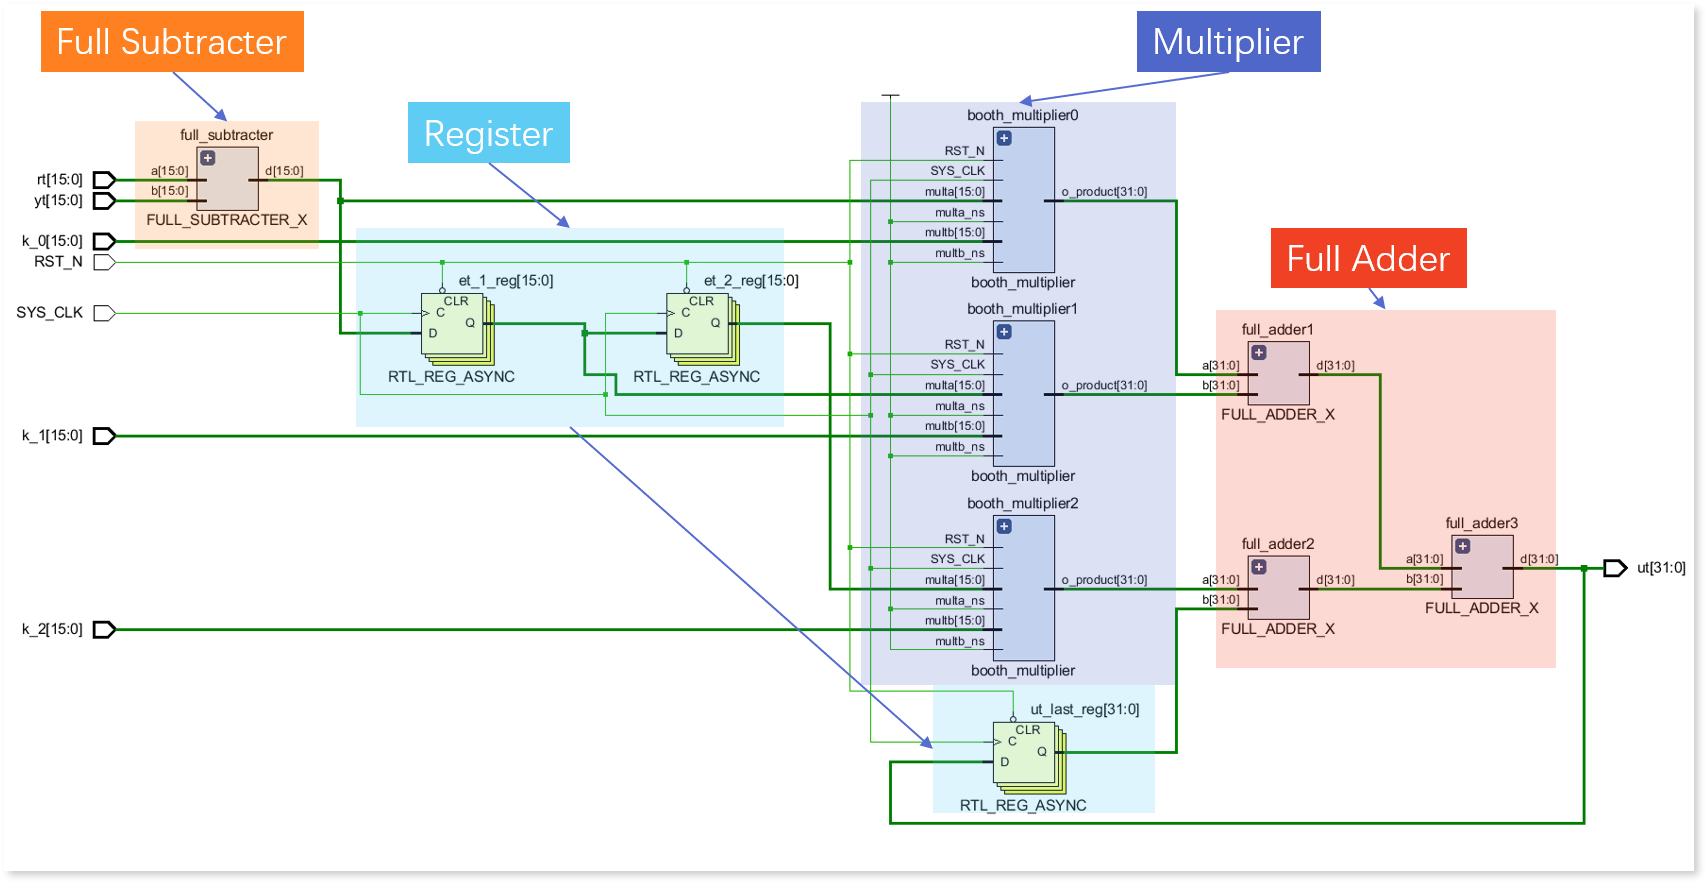
\includegraphics[width=1.0\linewidth]{rtmq/digital_pid_structure_16bits}
\end{figure}

整个PID控制器使用了一个减法器、三个加法器、三个乘法器和若干寄存器。图\ref{fig:digital_pid_structure_16bits}是一个16位输入的数字PID,它的输出是32位的,该实例模块总共包含9级流水线,工作频率可达200MHz以上。对更低或者更高位数的数字PID控制器,可以通过替换相应位数的加减运算和乘法模块,并调整相应的寄存器位宽来方便地得到。




\newpage
\section[基于FPGA的通用数字滤波器]{基于FPGA的通用数字滤波器\label{section:digital_iir}}
滤波器是一种选频装置,可以使信号中特定的频率成分通过,而极大地衰减其它频率成分。利用滤波器的这种选频作用,可以滤除干扰噪声或进行频谱分析。数字滤波器是一个离散时间系统,其输入、输出都是离散时间信号,它是通过对输入信号进行一定的运算处理,从而达到对信号进行滤波的目的。数字滤波器可以分为经典滤波器和现代滤波器两类。
 
经典滤波器是假定输入信号$x(n)$中的有用成分和希望去除的成分各自占有不同的频带,当通过一个线性系统后即可将欲去除的成分有效地去除。在经典滤波器中,输入信号被分成不同的频带,然后通过一个低通滤波器或高通滤波器来实现滤波。
 
现代滤波器是根据信号的随机过程模型,利用统计最优准则设计的一类滤波器。现代滤波器可以分为维纳滤波器、卡尔曼滤波器、自适应滤波器等。它们的共同特点是能够从含有噪声的数据中有效地提取信号,同时抑制噪声。


\subsection[数字滤波器]{数字滤波器}
% \textcolor{red}{
% 1. 介绍数字滤波器功能、种类、基本原理,比如有限冲激响应滤波器、无限冲激响应滤波器等等;}

数字滤波器的基本原理是利用离散系统的特性对输入信号进行加工和处理,改变输入信号的频率特性,从而达到选频、提高信噪比、消除干扰等目的。数字滤波器一般由延迟单元、加法器、乘法器、寄存器等基本运算单元组成。
 
不同类型的数字滤波器有不同的实现方法和应用领域。在通信、语音处理、图像处理、信号处理等领域,数字滤波器都有着广泛的应用。整个离子阱系统中很多模块都有滤波器的需求以获取更高质量的信号来控制量子比特。为此,整个RTMQ系统中需要实现数字滤波器以供系统设计和实现使用。



\subsection[无限冲激响应滤波器IIR]{无限冲激响应滤波器IIR}
有限冲击响应滤波器(FIR滤波器)的冲激响应在有限时间内衰减为零,其输出仅取决于当前和过去的输入信号值。FIR滤波器在保证幅度特性的同时,很容易做到严格的线性相位特性。无限冲击响应滤波器(IIR滤波器)的冲激响应理论上应会无限持续,其输出不仅取决于当前和过去的输入信号值,也取决于过去的信号输出值。

有限冲击响应滤波器(FIR滤波器)的优点是具有线性相位、稳定性好、容易实现等,缺点是阶数较高时,运算量较大,对存储空间要求较高。无限冲击响应滤波器(IIR滤波器)的优点是阶数较低时,运算量较小,对存储空间要求较低,缺点是相位非线性、稳定性较差、设计复杂等。实际滤波器设计经验表明,实现相同形状的滤波效果,IIR滤波器所需的计算资源远小于FIR滤波器。鉴于硬件实现是对资源十分敏感的,因此我们选用IIR滤波器来进行实现。

IIR滤波器的冲激响应理论上应会无限持续,其输出不仅取决于当前和过去的输入信号值,也取决于过去的信号输出值,用差分方程来表示一个滤波器,其表达式为:
\begin{align}
    y(n)=\sum_{k=1}^Na_ky(n-k)+\sum_{k=0}^Nb_kx(n-k)\label{eq:iir_filter}
\end{align}

 % \textcolor{red}{
% 2. 介绍数字通用滤波器功能、逻辑图、Vivado中的实现、优势;}

其中,$y(n)$表示输出信号,$x(n)$表示输入信号,$a_k$和$b_k$表示滤波器系数。本质上来说,IIR滤波器就是将输入和过去的输出按照某种方式加权计算获得最终输出结果的。对于一个给定阶数和数字位数的IIR滤波器,它的形状完全取决于系数$a_k$和$b_k$。因此,为了维持通用性,在硬件实现的过程中,我们应该把系数($a_k, b_k$)设计为可外部软件配置的。
以四阶为例,通用四阶IIR滤波器的结构框图如图\ref{fig:iir_filter_s}所示,图中$a_0-a_3, b_0-b_3$为IIR滤波器的可配置系数,主要用到的模块有寄存器、乘法器、加法器等。
\begin{figure}
    \centering
    \caption[IIR滤波器结构框图]{IIR滤波器结构框图\label{fig:iir_filter_s}}
    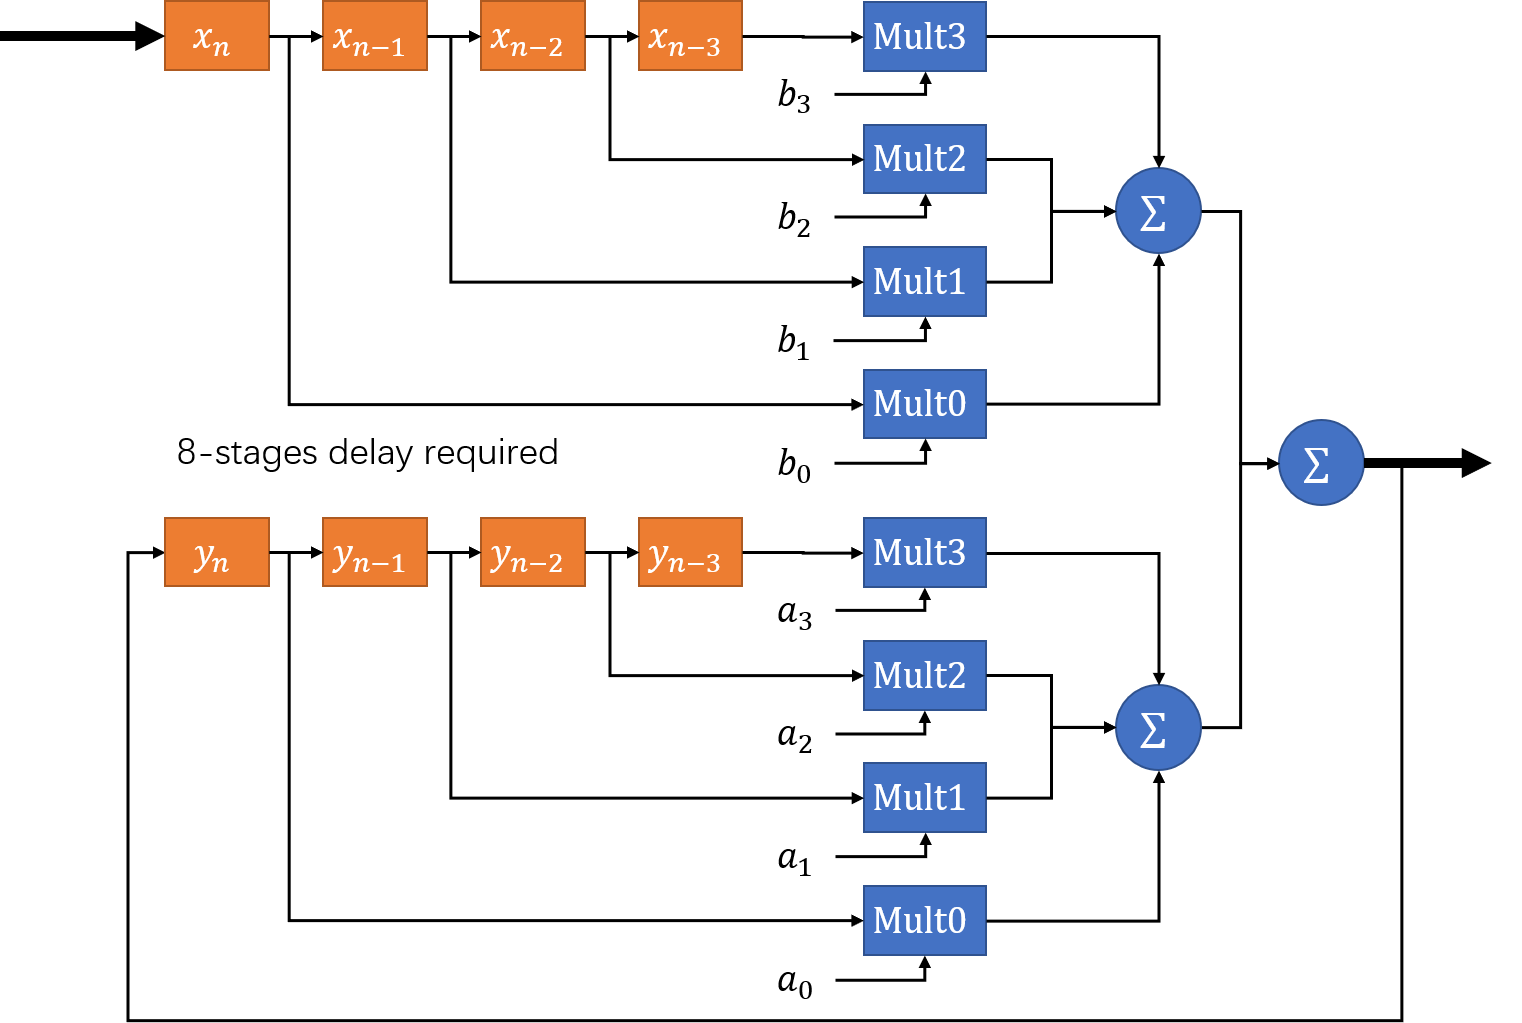
\includegraphics[width=1.0\linewidth]{rtmq/iir_filter_s}
\end{figure}


\subsection[数字IIR滤波器的FPGA实现]{数字IIR滤波器的FPGA实现}

根据图\ref{fig:iir_filter_s}给出的结构图和公式\eqref{eq:iir_filter},可以将其在FPGA中进行实现和验证。数字IIR滤波器在FPGA中的实现结果的结构图如图\ref{fig:iir_filter_vivado}所示,整体结构中超如了若干的流水线用于对齐$x(n)$和$y(n)$的时序。除此之外,流水线也被用于满足电路的时延要求。需要注意的是,由于上一时刻的输出结果$y(n-1)$需要参与到下一时刻的输出结果的计算中,因此从计算结果到迭代反馈之间仅能有一级流水线存在,否则输出结果就会出错。也正因此,这个IIR滤波器无法工作在较高的频率上,需要在板上额外配置工作频率,该32位通用IIR滤波器设计在FPGA板上的工作频率为25MHz。

\begin{figure}
    \centering
    \caption[IIR滤波器实现结果的结构图]{IIR滤波器实现结果的结构图(Vivado)\label{fig:iir_filter_vivado}}
    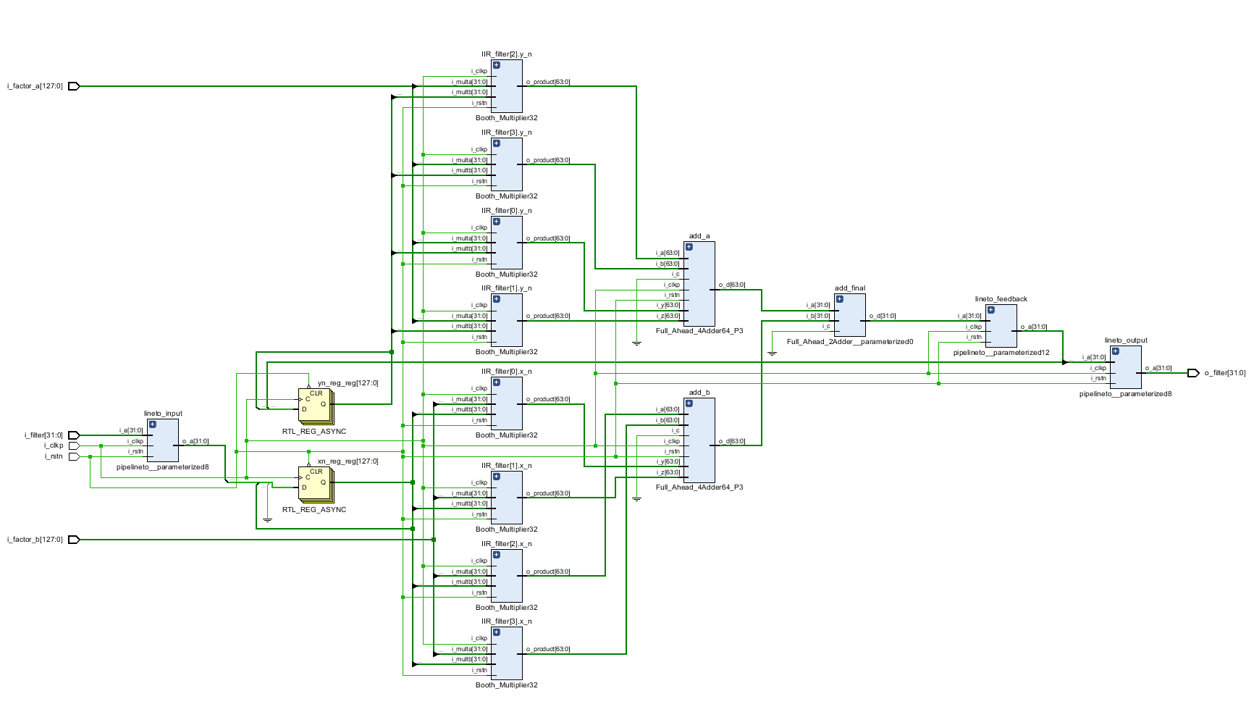
\includegraphics[width=1.0\linewidth]{rtmq/iir_filter_vivado}
\end{figure}




\subsection[滤波器形状测量]{滤波器形状测量}
数字滤波器的形状设计可以采用MATLAB中的滤波器设计器来完成。在量子计算的试验系统中常常要应对的是高频信号噪声,低通滤波器是十分常见的需求,因此下面以低通滤波器为例进行说明。如图\ref{fig:filter_design_real1},通过MATLAB设计了一个截止频率在100kHz附近的巴特沃斯型迭代滤波器,结果为一个3阶的迭代滤波器,参数为:$a_0=16777216;
a_1=-33470572;
a_2=16693565;
a_3=0;
b_0=52;
b_1=105;
b_2=52;
b_3=0$。可以看到设计的理论截止频率(100kHz)和数字滤波器实际的截止频率(13.17kHz)有较大的差异。其原因主要有两方面:1. 数字滤波器的设计本身实际上是对模拟滤波器的近似,因而结果不绝对准确;2. 实际在FPGA中的硬件滤波器运算位宽有限,爹地啊过程中存在截断效应;3. 对数据的表征不够精确,测试的过程中用到模数转换(16位)等中间数字过程。

\begin{figure}
    \centering
    \caption[IIR滤波器设计仿真和实际测试结果]{IIR滤波器设计仿真和实际测试结果\label{fig:filter_design_real1}}
    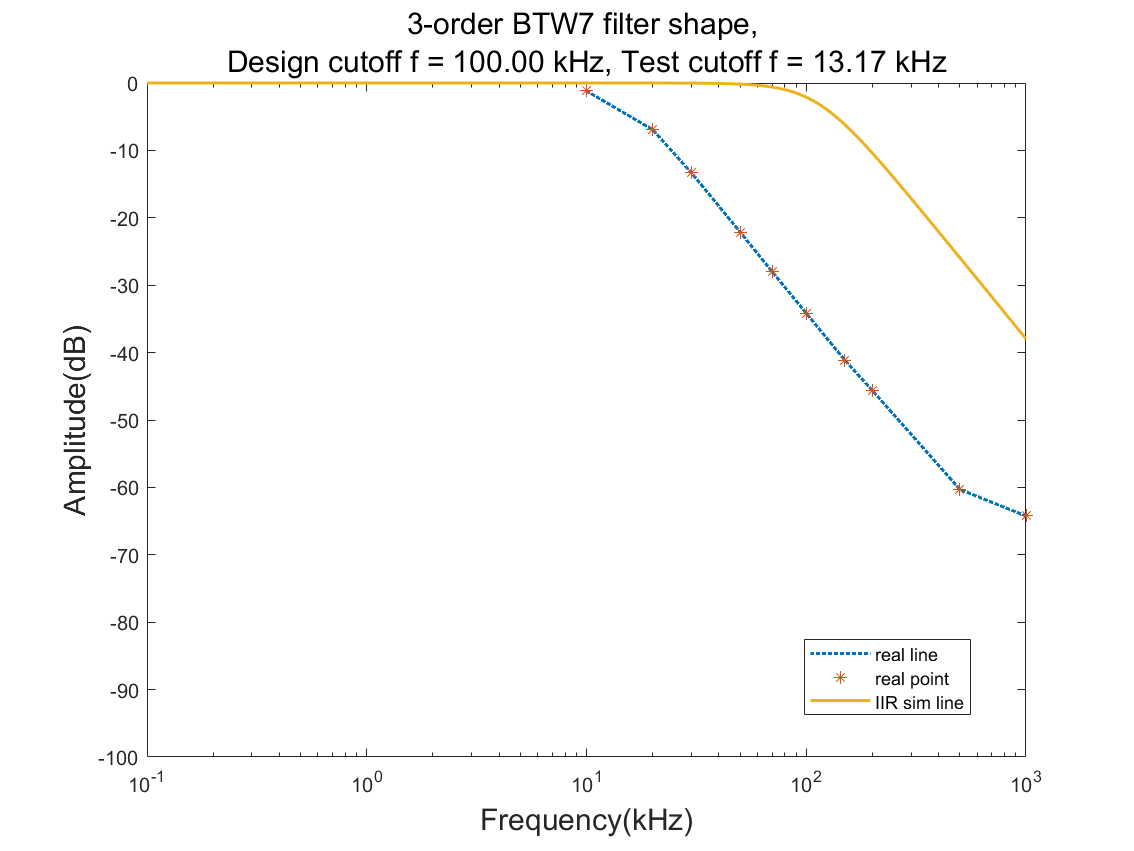
\includegraphics[width=1.0\linewidth]{rtmq/filter_design_real1}
\end{figure}

在理论结果绘制中,对滤波器的结果进行类似FPGA硬件中的人工截断,得到的模拟结果如图\ref{fig:filter_design_real2}所示。可以看到此时理论设计的截止频率结果与实际硬件数字PID的截止频率结果变得更加接近了。尽管仍然存在一定的差异,已经可以给出比较有意义的指导信息了。整体上来看,硬件实现的数字滤波器在配置为低通滤波器的时候带宽会被压窄。因此如果需要100kHz的带宽,则需要在设计时适当放大这个带宽需求。最终实际的滤波器带宽可以通过测量来进一步验证是否符合使用要求,如果不符合则可以重新设计和测试。值得一提的是,在实现了通用的硬件IIR滤波的基础上,重新设计和配置$a_0-a_3, b_0-b_3$等参数是十分方便快捷的,仅需更改可配置寄存器的值即可。

\begin{figure}
    \centering
    \caption[IIR滤波器考虑截断的仿真和实际测试结果]{IIR滤波器考虑截断的仿真和实际测试结果\label{fig:filter_design_real2}}
    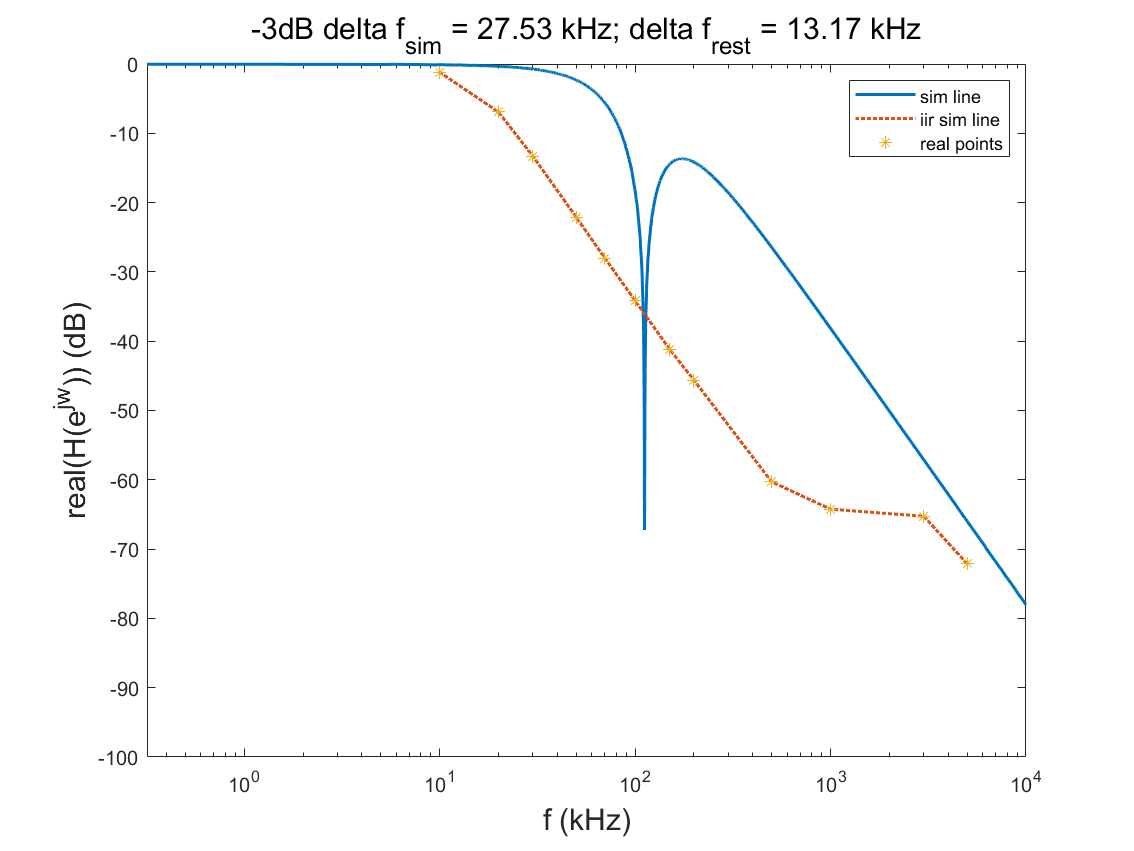
\includegraphics[width=1.0\linewidth]{rtmq/filter_design_real2}
\end{figure}

% IIR滤波器形状测量如图\ref{fig:iir_filter_shape}所示。
% \begin{figure}
%     \centering
%     \caption[IIR滤波器设计仿真和不同参数下测试结果]{IIR滤波器设计仿真和不同参数下测试结果\label{fig:iir_filter_shape}}
%     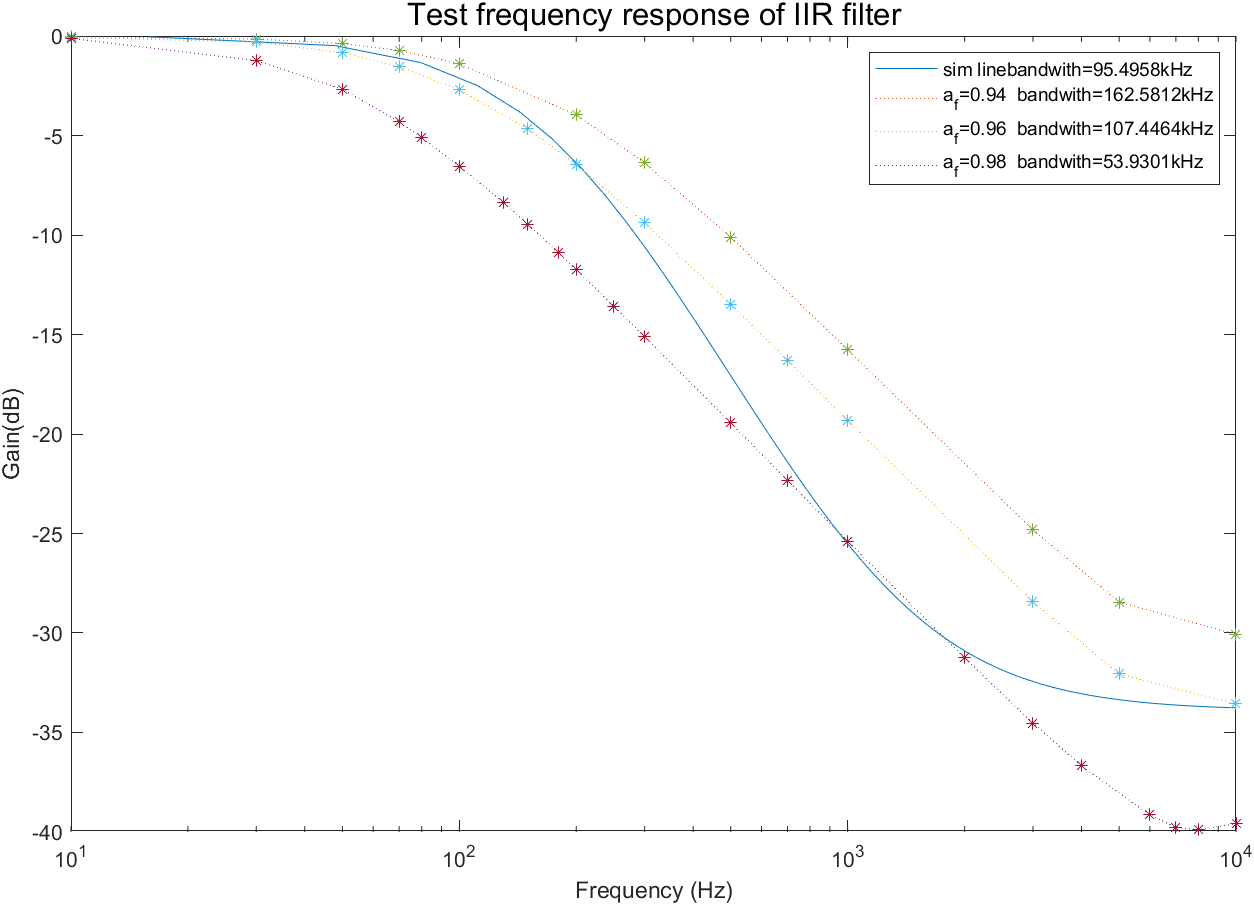
\includegraphics[width=1.0\linewidth]{rtmq/iir_filter_shape}
% \end{figure}